% Options for packages loaded elsewhere
\PassOptionsToPackage{unicode}{hyperref}
\PassOptionsToPackage{hyphens}{url}
\PassOptionsToPackage{dvipsnames,svgnames,x11names}{xcolor}
%
\documentclass[
  10pt,
  twocolumn]{aft}

\usepackage{amsmath,amssymb}
\usepackage{iftex}
\ifPDFTeX
  \usepackage[T1]{fontenc}
  \usepackage[utf8]{inputenc}
  \usepackage{textcomp} % provide euro and other symbols
\else % if luatex or xetex
  \usepackage{unicode-math}
  \defaultfontfeatures{Scale=MatchLowercase}
  \defaultfontfeatures[\rmfamily]{Ligatures=TeX,Scale=1}
\fi
\usepackage{lmodern}
\ifPDFTeX\else  
    % xetex/luatex font selection
\fi
% Use upquote if available, for straight quotes in verbatim environments
\IfFileExists{upquote.sty}{\usepackage{upquote}}{}
\IfFileExists{microtype.sty}{% use microtype if available
  \usepackage[]{microtype}
  \UseMicrotypeSet[protrusion]{basicmath} % disable protrusion for tt fonts
}{}
\makeatletter
\@ifundefined{KOMAClassName}{% if non-KOMA class
  \IfFileExists{parskip.sty}{%
    \usepackage{parskip}
  }{% else
    \setlength{\parindent}{0pt}
    \setlength{\parskip}{6pt plus 2pt minus 1pt}}
}{% if KOMA class
  \KOMAoptions{parskip=half}}
\makeatother
\usepackage{xcolor}
\usepackage[top=2.5cm,bottom=2.5cm,left=1.5cm,right=1.5cm,heightrounded]{geometry}
\setlength{\emergencystretch}{3em} % prevent overfull lines
\setcounter{secnumdepth}{5}
% Make \paragraph and \subparagraph free-standing
\ifx\paragraph\undefined\else
  \let\oldparagraph\paragraph
  \renewcommand{\paragraph}[1]{\oldparagraph{#1}\mbox{}}
\fi
\ifx\subparagraph\undefined\else
  \let\oldsubparagraph\subparagraph
  \renewcommand{\subparagraph}[1]{\oldsubparagraph{#1}\mbox{}}
\fi


\providecommand{\tightlist}{%
  \setlength{\itemsep}{0pt}\setlength{\parskip}{0pt}}\usepackage{longtable,booktabs,array}
\usepackage{calc} % for calculating minipage widths
% Correct order of tables after \paragraph or \subparagraph
\usepackage{etoolbox}
\makeatletter
\patchcmd\longtable{\par}{\if@noskipsec\mbox{}\fi\par}{}{}
\makeatother
% Allow footnotes in longtable head/foot
\IfFileExists{footnotehyper.sty}{\usepackage{footnotehyper}}{\usepackage{footnote}}
\makesavenoteenv{longtable}
\usepackage{graphicx}
\makeatletter
\def\maxwidth{\ifdim\Gin@nat@width>\linewidth\linewidth\else\Gin@nat@width\fi}
\def\maxheight{\ifdim\Gin@nat@height>\textheight\textheight\else\Gin@nat@height\fi}
\makeatother
% Scale images if necessary, so that they will not overflow the page
% margins by default, and it is still possible to overwrite the defaults
% using explicit options in \includegraphics[width, height, ...]{}
\setkeys{Gin}{width=\maxwidth,height=\maxheight,keepaspectratio}
% Set default figure placement to htbp
\makeatletter
\def\fps@figure{htbp}
\makeatother

\usepackage{multirow}
\usepackage{array}
\usepackage{longtable}
\usepackage{multicol}
\usepackage{caption}
\usepackage{rotating}
\usepackage{pdflscape}
\usepackage{float}
\usepackage{fontspec}
\usepackage{threeparttable}
\captionsetup{justification=justified,singlelinecheck=false}
\usepackage[LGRgreek]{mathastext}
\usepackage{mathtools}
\usepackage{orcidlink}
\definecolor{mypink}{RGB}{219, 48, 122}
\makeatletter
\@ifpackageloaded{caption}{}{\usepackage{caption}}
\AtBeginDocument{%
\ifdefined\contentsname
  \renewcommand*\contentsname{Table of contents}
\else
  \newcommand\contentsname{Table of contents}
\fi
\ifdefined\listfigurename
  \renewcommand*\listfigurename{List of Figures}
\else
  \newcommand\listfigurename{List of Figures}
\fi
\ifdefined\listtablename
  \renewcommand*\listtablename{List of Tables}
\else
  \newcommand\listtablename{List of Tables}
\fi
\ifdefined\figurename
  \renewcommand*\figurename{Figure}
\else
  \newcommand\figurename{Figure}
\fi
\ifdefined\tablename
  \renewcommand*\tablename{Table}
\else
  \newcommand\tablename{Table}
\fi
}
\@ifpackageloaded{float}{}{\usepackage{float}}
\floatstyle{ruled}
\@ifundefined{c@chapter}{\newfloat{codelisting}{h}{lop}}{\newfloat{codelisting}{h}{lop}[chapter]}
\floatname{codelisting}{Listing}
\newcommand*\listoflistings{\listof{codelisting}{List of Listings}}
\makeatother
\makeatletter
\@ifpackageloaded{caption}{}{\usepackage{caption}}
\@ifpackageloaded{subcaption}{}{\usepackage{subcaption}}
\makeatother
\makeatletter
\makeatother
\ifLuaTeX
  \usepackage{selnolig}  % disable illegal ligatures
\fi
\usepackage[]{natbib}
\bibliographystyle{apalike}
\IfFileExists{bookmark.sty}{\usepackage{bookmark}}{\usepackage{hyperref}}
\IfFileExists{xurl.sty}{\usepackage{xurl}}{} % add URL line breaks if available
\urlstyle{same} % disable monospaced font for URLs
\hypersetup{
  pdftitle={Local drivers and global suppliers of GHG emissions from the city of Madrid, 2010-2021},
  pdfauthor={Jacobo Ferrer; Sergio Alvarez},
  pdfkeywords={carbon footprint, input-output, cities, mitigation
planning, scope 3},
  colorlinks=true,
  linkcolor={blue},
  filecolor={Maroon},
  citecolor={Blue},
  urlcolor={blue},
  pdfcreator={LaTeX via pandoc}}


\begin{Huge}
\title{Local drivers and global suppliers of GHG emissions from the city
of Madrid, 2010-2021\footnote{a}}
\end{Huge}
\author{
Jacobo Ferrer~\orcidlink{0000-0002-7873-6275}\\Universidad Politécnica
de
Madrid\\Contact at: \href{mailto:jacobo.ferrer@upm.es}{jacobo.ferrer@upm.es}\\\and 
Sergio Alvarez~\orcidlink{0000-0001-7204-502X}\\Universidad Politécnica
de
Madrid\\Contact at: \href{mailto:sergio.alvarez@upm.es}{sergio.alvarez@upm.es}\\}
\date{Thursday, November 14, 2024}
\begin{document}

\makeatletter
\twocolumn[
\maketitle

\begin{@twocolumnfalse}

\centering\begin{minipage}{\dimexpr\paperwidth-6.5cm}
\begin{abstract}
\begin{normalsize}
% Write your abstract here ----------------------------------------------------
\vspace{1em}
Urban economies bear a significant responsibility in climate change, but estimating scope-3 emissions of urban areas is challenging due to the lack of city-level input-output tables and air emissions accounts. These limitations have led to various bottom-up and top-down strategies to address the information gap, often relying on the adoption of stringent domestic input-output modeling assumptions that limit considerably the analytical scope and granularity of the results. This paper presents the most rigorous quantification of the 3-scope carbon footprint of the city of Madrid to date, a full 2010-2021 series with a 28-industry and 47-country breakdown. The methodology consists in, firstly, integrating municipal-level economic data with regional supply and use tables to construct a series of city-specific input-output tables and to incorporate them into the FIGARO global multiregional input-output framework; secondly, constructing the first air emissions account for the city of Madrid, including direct emissions by households; thirdly,deriving a final consumption expenditure vector from household surveys. Our analysis reveals that the city's carbon footprint in 2021 was 17,447 ktCO2e for GDP and 13,920 ktCO2e for households. Only 15\% originated within the city limits, 34\% from the rest of Spain, and 51\% from the rest of the world. The analytical possibilities offered by these data are considerably broad. We find significant emissions inequality among residents, with the top 20\% of the equivalized spending distribution emitting 4.8 times more than the bottom 20\%. %
Structural decomposition analysis shows that while efficiency improvements and technological advancements contributed to emissions reduction, these gains were largely offset by increases in consumption demand. 
Notably, our simulations indicate that reshaping consumption patterns of higher-income households could potentially reduce emissions by up to 26\%, which is similar to the potential emissions savings from a substantial shift modality in private transport. The study underscores the need for consumption-oriented mitigation strategies and highlights the importance of addressing emissions inequality in urban climate action plans.
\end{normalsize}
\end{abstract}
\begin{flushleft}
\setlength\parindent{30pt}{
\hspace{\parindent}\small\textbf{Keywords}: {carbon footprint,
input-output, cities, mitigation planning, scope 3}.}
\end{flushleft}
\end{minipage}

\vspace{3em}
\end{@twocolumnfalse}]
\makeatother
\section{Introduction}\label{sec-introduction}

According to the IPCC Sixth Assessment Report, policy implementation
will likely fall short of the carbon dioxide (\(CO_2\)) emissions
targets implied in the Nationally Determined Contributions (NDCs) of the
Paris Agreement announced ahead of the UN Climate Change Conference
(COP26) \citep{ipcc_summary_2022}. Under the current scenario, limiting
global warming to below 2°C will require a~rapid acceleration of
mitigation efforts in overall fossil fuel use after 2030. Such
transformation will require drastic reductions in industry emissions for
which sector-specific interventions may prove insufficient without
substantial changes to consumption and mobility patterns
\citep{ipcc_summary_2023}. For this purpose, urban areas are uniquely
positioned to contribute to this type of mitigation efforts. Cities are
responsible for a significant proportion of \(\text{CO}_2e\) emissions
\citep{ipcc_climate_2023, wiedmann_city_2021, hoornweg_cities_2011} and,
with global urban population at 56\% and projected to host more than
70\% in 2050 \citep{un_world_2022}, its weight on decarbonization
responsabilities will only continue to grow.

In the European context, Madrid is the second-largest metropolitan area
of the European Union with over 6 million people
\citep{eurostat_population_2024}. It is also one of the fastest-growing
economic regions in Southern Europe \citep{eurostat_gross_2024}. At the
center is the city of Madrid, which in 2022 had a population of 3.28
million inhabitants (6.9\% of the country and 48\% of the region),
reached a GDP of \euro{}168 billion (12.7\% of the Spanish GDP), and a
per capita GDP of \euro{}51466
\citep{am_areas_2023, amMadridEconomia20232023}. The service sector
dominates the local economy (88.3\%), specially in industries such as
professional business activities, tourism, and trade, and it hosts only
a modest amount of manufacturing activity (7.4\%)
\citep{am_areas_2023, am_estructura_2013, amRoadmapClimateNeutrality2022, amMadridEconomia20232023}.
It has few sources of primary energy, with no fossil fuel reserves or
energy transformation plants, but a substantial level of energy
consumption \citep{perez_methodology_2019}. The economic and demographic
scale of the city make its firms and households fundamental drivers of
direct and indirect \(\text{CO}_2e\) emissions in Spain.

The City Council has repeatedly stated its commitment to tackling
climate change \citep{am_inventario_2021}. After several plans guiding
mitigation and adaptation interventions, the City Council approved the
\emph{Roadmap towards Climate Neutrality for 2050} (the Roadmap,
hereafter) \citep{amRoadmapClimateNeutrality2022}, which lays out a
comprehensive plan to meet the objectives of the Paris Agreement and the
EU Climate Agenda \citep{JRC130230}. In particular, the ``Roadmap aims
at reducing emissions in the city of Madrid by 65\% by 2030, as compared
to 1990, and to achieve climate neutrality by 2050''
\citep[p.3]{amRoadmapClimateNeutrality2022}. If direct emissions totaled
12954 \(\text{ktCO}_2e\) in 1990, this means that they should fall below
4534 \(\text{ktCO}_2e\) by 2030
\citep[12]{amRoadmapClimateNeutrality2022}. To monitor this evolution,
the City Council produced the local \emph{Air Pollutant Emissions
Inventory} in addition to the \emph{Energy Balance} of the municipality
of Madrid. The Air Emissions Inventory (AEI) provides information for
over two decades on ``direct emissions (scope 1) and indirect emissions
due to electricity consumption and distribution losses (scopes 2 and 3),
broken down by sector of activity''
\citep[p.6]{amRoadmapClimateNeutrality2022}. This complex piece of
information has been a crucial contribution to the quantification of the
city's responsability in climate change, as well as an indispensable
tool to evaluate the implementation of mitigation policies, specifically
the Roadmap. According to the Council, these data indicate that Madrid
seems on track to meet its mitigation goals within a conservative
`sustainable' scenario
\citep{JRC130230, amRoadmapClimateNeutrality2022}.

Consequently, the construction of a city scale AEI have been an
invaluable first step toward achieving \emph{direct} \(\text{CO}_2e\)
emissions reduction in Madrid. Nevertheless, we know that
\emph{indirect} emissions tend not only to be larger than direct
emissions, but also grow in time as countries or cities transition
towards a highly tertiarize economy. In the 2010s, coinciding with a
growing number of cities setting net-zero emissions targets and
producing \(\text{CO}_2e\) inventories using standard protocols, a
literature studying the carbon footprint (CF) of cities started to
quantify the extent of transboundary emissions
\citep{wiedmann_city_2021}. These studies have shown time and again that
direct emissions are but a fraction of the total CF of any urban area
\citep{wiedmann_threescope_2021, wiedmann_city_2021, c40_future_2019, eea_environmental_2013}.
Since cities have offshored most of its energy production and
manufacturing activity, so it has the \(\text{CO}_2e\) emissions
requirements embodied in those imports \citep{wiedmann_threescope_2021}.
The notion of emissions scopes separates clearly the visible from the
invisible part of any CF. If inventories account for scope-1 or direct
emissions, scopes-2 and -3 reflect the full carbon responsability of
economic and domestic choices. In particular, scope-3 or embedded
emissions are the hardest to quantify, but they account for the lion's
share of the contribution to climate change
\citep{creutzig_demand-side_2022, wiedmann_city_2021, chen_urban_2020, moran_carbon_2018, ivanova_mapping_2017, wiedmann_concept_2016, kennedy_egregious_2014}.
According to \citet[p.~16]{c40_future_2019}, around 85\% of the
consumption-based GHG emissions of C40's 94 members are generated
outside the city boundaries, which influeces close to 10\% of global
emissions. Thus, increasing our knowledge about the geographical
distribution of outsourced emissions is crucial to properly quantify
cities' indirect emissions
\citep{wiedmann_threescope_2021, eea_environmental_2013}. Furthermore,
by differentiating the geographical origin of emissions, we can identify
possible international constraints on decarbonization ambitions
\citep{remond-tiedrez_eu_2019}.

City CFs show a particularly large discrepancy between production-based
and consumption-based estimations \citep{c40_future_2019}. In addition
to being substantially more open than countries to cross-boundary
exchanges of material and financial flows, cities are richer on average
\citep{wiedmann_city_2021}. The level of per capita consumption is
closely correlated with total consumption-based emissions
\citep{wiedmann_threescope_2021, lopez_how_2017, eea_environmental_2013}.
Inequality contributes to shape the urban emissions profile by
introducing heterogeneity in demand
\citep{chancelClimateInequalityReport2023, lopez_how_2017}. A well-known
stylized fact of consumption is that the weight of essentials on family
budgets, such as the amount spent on food or heating, declines as a
function of the level of real income
\citep{browningEngelLaw2018, kausEngelLawCrosscountry2013, chaiBackEngelEvidence2013}.
Hence, different levels of inequality will introduce non-linear
variations in total emissions as real income grows
\citep{levinsonEnvironmentalEngelCurves2015}. Urban consumption patterns
are not only heterogenous but also distinctive vis-à-vis rural areas
\citep{lopez_assessing_2016, wiedmann_city_2021}, which controlling for
the level of spending tend to be less \(\text{CO}_2e\) intensive
\citep{corcoles_carbon_2024, lopez_assessing_2016}. This have been
connected to household's private transport and heating/cooling use
\citep{corcoles_carbon_2024}, which, given the economies of scale of
urban transport systems, invites further scrutiny over private mobility
choices. The combination of lifestyles, municipal regulation,
agglomeration economies, and infraestructure limitations shape the
peculiar structure of urban economies. Understanding the sources of
heterogeneity of consumption demand and economic activity in urban areas
are, thus, crucial to properly design mitigation and adaptation policies
\citep{ipcc_climate_2023}.

Although input-output analysis has been applied to cities for a long
time, the lack of tables at city scale have drawn many researchers to
use national coefficient tables and non-survey methods
\citep{wiedmann_concept_2016, fry_assessing_2018, wiedmann_city_2021, moran_carbon_2018}.
The substantial differences in the carbon intensity of city products and
activities often lead to overestimation of production-based CFs
depending on the weight of industrial activity in the city or the
institutional sectors included in the calculation
\citep{fry_assessing_2018}. On the other hand, the lack of city-scale
global multi-regional input-output tables (GMRIO) further distorts the
interconnections of the city with the rest of the world, increasing the,
often downward, bias in the estimation of consumption-based CFs.
Similarly to the literature working on regional CFs, this bias often
stems from the data quality compromises required to produce
simultaneously thousands of city footprints
\citep{moran_carbon_2018, caro_mapping_2017, eea_environmental_2013, ivanova_mapping_2017}.
The ability to focus on a single case opens the possibility to treat
sources more carefully, and bring external validation to more
comprehensive studies. Despite the availability of studies presenting
information for many cities including Madrid
\citep{andradeImplementingCitylevelCarbon2018, c40_consumption-based_2018, wiedmann_threescope_2021},
they either fail to exploit the full potential of available information
to improve estimation precision, or lack continuity and timeliness by
presenting out-of-date single-year estimations.

No coherent decarbonization target can be reached by offshoring the
emissions we are responsible for. Ignoring the accounting gap is
unacceptable given the committment displayed by the European Comission,
e.g.~the European Green Deal. Therefore, if local authorities are
comitted to come to grips with their decarbonization targets, they need
to quantify and factor the full scope of indirect emissions into their
mitigation planning. If indirect emissions are not factored into
decarbonization scenarios, we can be certain that a 65\% reduction of
emissions will not equal 4534 \(\text{ktCO}_2e\) in 2030, but a
substantially higher figure that is incompatible with the carbon
neutrality commitment by 2050. In this connection, the paper presents
the most precise and complete estimation to date of the structure and
evolution of Madrid's CF by looking at the supply and demand of
\(\text{CO}_2e\) emissions along the entire global value chain. It aims
to contribute to the growing literature on urban CFs by exemplifying the
analytical potential of using city-augmented models in combination with
household surveys to track the origin and characteristics of emissions
generation from the supply and the demand side
\citep{wiedmann_city_2021, chen_urban_2020, moran_carbon_2018, c40_consumption-based_2018}.
It aims to estimate and characterize the 3-scope CF of the city and to
break down its drivers and suppliers by geographical area, industry,
consumption purpose, and socio-demographic grouping. To do this, we
project a city industry-by-industry input-output table (IOT) exploiting
the regional supply and use framework (SUT) and 28-industry macro data
from the municipal economic accounts \citep{am_areas_2023}. We embed the
city table within the GMRIO framework provided by the \emph{Full
International and Global Accounts for Research in input-Output analysis}
(FIGARO) database \citep{remond-tiedrez_eu_2019} to obtain as much
geographical and industry detail as possible. We obtain city-level
emission factors by constructing an air emissions account (AEA) from the
city's inventory data \citep{am_inventario_2021} following Eurostat's
methodology \citep{eurostat_manual_2015, eurostat_european_2013}.
Consumption spending and socio-demographic information about city
residents come from the Spanish Household Budget Survey (ES-HBS), which
we use to derive a city consumption vector following the steps explained
by \citet{cazcarro_linking_2022}, as well as direct household emissions
related to heat and transport activities as in
\citet{corcoles_carbon_2024}. Additionally, we impute
individual-household \(\text{CO}_2e\) volumes by 3-digit consumption
purpose using aggregate emissions intensity per unit of nominal
spending, with which we are able to present a bird's-eye view of the
socio-demographic composition of the city's CF. Finally, we illustrate
the potential of trade vis-à-vis consumption for mitigation policy via
several emission reduction simulation scenarios based on supply chain
reconfiguration and household behavior.

The outline of the rest of the paper is as follows.
Section~\ref{sec-method} presents the sources and methods used to derive
the city-augmented GMRIO framework. In section \ref{sec-method-gmrio} we
briefly explain the computation method for the total CF in line with the
literature. Section \ref{sec-method-household} explains the information
requirements and methodological choices involved in the derivation of a
workable city final consumption vector using micro observations from the
ES-HBS. In section \ref{sec-method-city} we document the process by
which we construct a city input-output series from 2010 to 2021 to be
then included coherently within FIGARO, which includes the derivation of
the rest-of-the-nation and international requirement coefficients.
Section~\ref{sec-method-emissions} explains the construction of the city
AEA. Last for section \ref{sec-method}, \ref{sec-subsec-decomposition}
shows the methodology applied to obtain the structural decomposition of
the city's CF into an intensity, a trade, a technology, and consumption
level component, as well as how we are able to simulate changes to
global supply chains parsimoniously. Section~\ref{sec-results} presents
the empirical results, which separates the perspective of the city's
activity (GDP) in \ref{sec-subsec-results-gdp} from households'
consumption in \ref{sec-subsec-results-households} and from the
structural decomposition with the trade and consumption scenarios in
\ref{sec-decomposition-simulation}. In sections
\ref{sec-subsec-results-gdp} and \ref{sec-subsec-results-households} we
emphasize the geographical and group-wise (industry or consumption
purpose) distribution of embedded emissions, but it is in the latter
that we go in more depth about the distributional drivers of total
emissions from the perspective of household choices. We conclude with a
section \ref{sec-implications} discussing the main takeaways,
implications, and limitations of the empirical results.

\section{Methodology and sources}\label{sec-method}

\subsection{An GMRIO model for Scope-3 CF
estimation}\label{sec-method-gmrio}

The methodology for estimating CFs by means of environmentally extended
input-output models (EEIO) is well-supported by an extensive literature
\citep{miller_input-output_2022, ivanova_mapping_2017, eurostat_manual_2015, eea_environmental_2013, martinezIdentifyingEnvironmentalFootprint2019}.
The use of GMRIOs to distribute emissions along the global value chain
further expands out ability to pin down the geografical origin of
locally triggered emissions
\citep{wiedmann_threescope_2021, wiedmann_concept_2016, remond-tiedrez_eu_2019}.
Any CF can be calculated using the standard Leontief-inverse demand-pull
input-output model shown in Equation~\ref{eq-carbon-footprint}.
\begin{equation}\phantomsection\label{eq-carbon-footprint}{
CF^p = \hat{\textbf{e}}(\textbf{I} - \textbf{A})^{-1}\hat{\textbf{y}} 
}\end{equation}

where \(\hat{\textbf{e}}\) is the diagonalized \(1 \times n\) vector of
emission factors. The Leontief inverse
\((\textbf{I} - \textbf{A})^{-1}\) is a \(n \times n\) total
requirements matrix indicating the amount of inputs from the \(n\)
industries directly and indirectly required per unit of industry's \(j\)
output. The vector \(\hat{\textbf{y}}\) is the \(n \times 1\) final
demand vector, which can also be a diagonalized (\(n \times n\)) or
simply spread by the different demand components (\(n \times d\)), such
as households' final consumption or government spending. In the case of
a GMRIO, the dimensions span \(m\) number of regions or countries, such
that the Leontief inverse becomes an \(mn \times mn\) matrix, and
\(\textbf{e}^t\) and \(\textbf{y}\) \(mn \times 1\) vectors. One
advantage of diagonalizing a unique final demand vector
\(\hat{\textbf{y}}\), regardless of it being final consumption or gross
domestic product, is that it preserves the dimensions of the Leontief
inverse and, thus, allows for a row-wise or column-wise perspective,
depending on whether a supplier or driver approach is followed. The
latter corresponds to the CF concept used henceforth.

The paper will present two different approaches as we select the city's
GDP or households as our unit of analysis. On the one hand, we are
interested in the bi-dimensional distribution of emissions by source
industry and country of origin that the gross domestic product of the
city of Madrid is responsible for. From this perspective, the unit of
analysis is the domestic economic activity of the urban area, and it is
bounded by the National Accounts rules determining what counts as
economically meaningful activity
\citep{lequiller_understanding_2014, eurostat_european_2013}. On the
other, we also want to investigate the emissions produced by households.
These do not only include the direct and indirect emissions driven by
household final consumption expenditure, but also those originating in
heating, cooling, transportation or other household activities, which
fall outside of market-oriented production. In the case of households,
the \(CF^h\) will be a combination of the emissions embedded in the
goods and services purchased by households (\(CF^p\)) and those direct
\(\text{CO}_2e\) emissions originated in their direct domestic activity
(\(CF^d\)), which is divided in three different categories:
transportation, heating/cooling, and other fugitive emissions.
\begin{equation}\phantomsection\label{eq-carbon-footprint-households}{
CF^h =  CF^d + CF^p
}\end{equation}

We choose to derive symmetric industry-by-industry input-output tables
(IOTs) from the city-projected regional supply and use tables (RSUTs)
\citep{remond-tiedrez_eu_2019}, organized according to the second
revision of the Statistical Classification of Economic Activities in the
European Community (NACE). However, we will move from
industry-by-industry to product-by-product according to the Statistical
classification of Products by Activity (CPA) as required by the
necessary transformations applied to consumption microdata
\citep{miller_input-output_2022, cazcarro_linking_2022}. Whereas for
GDP-related emissions it suffices to match the classification matrix and
the emissions factors, results for household consumption come only after
additional steps.

\subsection{A city-augmented FIGARO-GMRIO}\label{sec-method-city}

\begin{figure*}

\centering{

\includegraphics[width=0.9\textwidth,height=\textheight]{graphics/Diagrama.pdf}

}

\caption{\label{fig-diagram}City-augmented GMRIO structure. Source:
Authors' own elaboration.}

\end{figure*}%

For the GMRIO framework, we rely on the global multi-regional supply and
use tables (GMSUTs) provided in the \emph{Full International and Global
Accounts for Research in input-Output analysis} (FIGARO) database
\citep{remond-tiedrez_eu_2019}, which is an official EU statistics
produced jointly by Eurostat and the Joint Research Centre of the
European Commission. In its current 2024 edition, FIGARO covers the
whole time series from 2010 to 2022 for the 27 EU Member States, the
United Kingdom, the United States and another 17 main EU partners, plus
a ``rest of the world'' region.

Following a series of authors \citep[e.g.][ and
\citet{wiedmann_threescope_2021}]{corcoles_carbon_2024}, we understand
how crucial is to balance practicality, granularity, and accuracy in the
production of city CFs. In this regard, we go beyond using national
tables and emission factors to approximate smaller territorial units,
for which direct observations are lacking. At the same time, we retain
the detailed information provided by the national database by embedding
the new tables within global value chains. This paper expands the
available FIGARO-GMRIO to include a symmetric input-output table of the
city of Madrid, with the corresponding adjustment to the rest of the
nation. Our approach takes inspiration from several contributions that
propose innovative non-survey methods to derive city-scale IOTs or SUTs
\citep[see][]{wiedmann_threescope_2021, moran_carbon_2018, zheng_entropy-based_2022, wiedmann_concept_2016}.
The three main data sources on which we produce our estimation are,
first, FIGARO's GMRIO 2010-2022 series, second, the RSUTs from the
region of Madrid covering the period from 2013 to 2019, and, third, the
municipal accounts data running from 2010 to 2022.
Figure~\ref{fig-diagram} describes the different elements involved in
the compilation of the city-augmented FIGARO-GMRIO database, where the
\textit{c}, \textit{n}, \textit{w} subscripts designate the city, the
rest of the nation (RoN), and the rest of the world (RoW), respectively.

To arrive at this result, we initially apply the GRAS algorithm, a
bi-proportional technique for updating IOTs with both positive and
negative elements
\citep{temurshoev_note_2013, lenzen_comments_2007, junius_solution_2003},
to the 2010-2021 series of RSUTs using as constraints the row and column
sums derived from the value added, intermediate input, and total output
vectors provided by the municipal industry accounts as shown in
equations \ref{eq-row-sums} and \ref{eq-column-sums} \vspace{-3pt}
\begin{equation}\phantomsection\label{eq-row-sums}{ b_i = x_i - \sum^k_{d=1} f_{i,d} }\end{equation}
\begin{equation}\phantomsection\label{eq-column-sums}{ b_j = x_j - \sum^r_{s=1} v_{s,j} }\end{equation}

where \(f_{i,d}\) are the \(k\), \(n \times 1\) vectors of final demand
components, \(v_{s,j}\) the \(r\) individual \(1 \times n\) vectors of
value-added subcomponents, typically gross operating surplus, total
labor compensation, and other taxes minus subsidies, \(x_i\) and \(x_j\)
are the \(n \times 1\) and \(1 \times n\) vectors of final output,
respectively, and \(b_i\) and and \(b_j\) are the \(n \times 1\) and
\(1 \times n\) summation vectors of the \(n \times n\) interindustry
transactions matrix \(\textbf{Z}=[z_{ij}]\). The vector of interindustry
row sums \(b_i\) is provided by the municipal accounts
\citep{am_areas_2023}, so only \(b_j\) has to be derived. Due to the
lack of information about the city's final demand, we obtain the final
demand vector \(f_i\) not by using equation \ref{eq-row-sums}, but by
multiplying the row sums of the regional direct requirement coefficients
times the municipal output vector. Furthermore, since the available
RSUTs series is smaller than our target FIGARO series, we use the 2013
RSUT for years 2010 to 2012, and the 2019 RSUT for years 2020 onwards as
templates for the missing coefficients.

As noted in the introduction, the region of Madrid is highly specialized
toward the service sector, with negligible contributions from
agriculture and only a modest one from manufacturing. Given this
constraint, we find that approximating the city table by means of the
regional table is almost certainly superior to using the national table.
On the other hand, since the municipal accounts data follows a
28-industry NACE (rev.2) classification, we first aggregate the regional
industry-by-industry symmetric table according to the municipal
classification. Thanks to a many-to-one relationship between the
regional and urban disaggregations, this poses no complication. Given
that the regional matrix distinguishes between domestic and imported
interindustry flows, we only need to aggregate both matrices to apply
the GRAS algorithm so that later we can separate the two using the
proportion of the original import flows to the corresponding domestic
ones. This way we can estimate the \(n \times n\) (n=28) interindustry
city matrix, defined as \(\textbf{Z}_{cc}\) in figure \ref{fig-diagram}.

Secondly, we need to estimate matrices \(\textbf{Z}_{cn}\) and
\(\textbf{Z}_{nc}\), which corresponds to the exports from the city to
the rest of the nation and the imports to the city from the rest of the
nation. From the import side, we have an interindustry import matrix
that we can use to separate the demand from the nation
\(\textbf{Z}_{nc}\) from that of the rest of the world
\(\textbf{Z}_{wc}\). To be efficient, we assume that the same proportion
of the national to the foreign value of each interindustry flow
\(z_{i,j}\) applies to the distribution of imports at the city level.
This assumes that firms in Madrid have the same incentive to purchase
inputs from the rest of the world as Spanish firms in general, which is
akin to a gravity assumption about extra-urban trade. Following
\citet[p.~475]{miller_input-output_2022}, we can obtain the total value
of imports from the rest of the nation \(z^{nc}_{i,j}\) as follows:
\vspace{-1.5pt}
\begin{equation}\phantomsection\label{eq-import-dist}{ z^{nc}_{i,j} = m^c_{i,j} - (m^n_{i,j}/z^n_{i,j}) = [1 - (m^n_{i,j}/z^n_{i,j})]m^c_{i,j}}\end{equation}

where \(m^c_{i,j}\) is the total city imports, \(m^n_{i,j}\) the total
national imports, and \(z^n_{i,j}\) the total value of domestic flows
from industry \(i\) to industry \(j\), respectively.

From the export side, we face additional difficulties to derive matrix
\(\textbf{Z}_{cw}\). Unlike in the case of imports, we lack a matrix of
export coefficients from industry \(j\) in the city to industry \(i\)
from the rest of the world. Furthermore, we have some concerns about the
reported values in the regional tables, as unlike any other macro
magnitude, they do not match the regional accounts provided by the
regional and the national statistical offices. The only relevant pieces
of information we preserve are the \emph{aggregate} trade balance and
the sectoral distribution of exports. We proceed, first, by adding up
the \emph{regional} trade balance to the city's import total to derive
the aggregate level of exports. We then multiply this total by the
industry export shares to apply the original distribution to the new
level. This way we can have a \(n \times 1\) vector of industry export
totals as in equation \ref{eq-export-dist}, \vspace{-3pt}
\begin{equation}\phantomsection\label{eq-export-dist}{ e^{c}_{i} = (e^{r^\ast} - m^{r^\ast})(e^r_{i}/\sum^n_{i=1}e^r_{i}) }\end{equation}

where \(e^{c}_{i}\) is the \(n \times 1\) vector of city export totals
by industry, \(e^r_{i}\) the equivalent vector from the regional table,
and \(e^{r^\ast}\) and \(m^{r^\ast}\) are the aggregate magnitude of
exports and imports at the regional level, respectively. Note that the
regional table is first of all transformed into industry-by-industry
IOTs and then aggregated to match the city industry classification.

At this point, we can apply the same procedure as in
Equation~\ref{eq-import-dist} to split the total between the rest of the
nation and the rest of the world. Basically, we multiply the level of
exports computed in the previous step by the share of domestic and
imported flows on total intermediate output from the Spanish national
table. This way we find a distribution between the rest of the nation
and the rest of the world assuming, again, that the pull from domestic
intermediate supplies is proportional to the demand that the city makes
from the rest of the nation. The full matrix of exports encompassing all
countries and sectors is found by premultiplying the diagonalized vector
of total industry exports to the rest of the world by the matrix of
industry export shares from Spain to the rest of the world, where the
normalizing constant is the total industry exports to the rest of the
world from the country. Finally, we obtain the rest-of-the-nation matrix
\(\textbf{Z}_{nn}\) by substracting matrices \(\textbf{Z}_{cc}\),
\(\textbf{Z}_{cn}\), and \(\textbf{Z}_{nc}\) from the original Spanish
national table, previously aggregated down to 28 industries to match the
municipal accounts.

Once all these pieces are ready, we can append them to the world
interindustry matrix. However, to produce fully-fledged IOTs, we include
the value added components from the city accounts (B2A3G, D29X39, and
D1, as per the SNA 2010 definition), adjusting the national vector
accordingly. We derive the vector of taxes minus subsidies on products
(D21X31, as per the SNA 2010 definition) by allocating proportionally
the national vector to the share of the city to the Spanish intermediate
flows total. Due to the limited information on final demand components
available in the city accounts, we decided to include only gross
domestic product (GDP), which for all countries can be derived from the
information available in FIGARO, final consumption of the household
sector (P3\_S14, as per the SNA 2010 definition), and final demand as
the sum of consumption and investment (P3AP5, as per the SNA 2010
definition). We perform several checks on the final matrix to make sure
that the totals from the new and the old matrix match for each
interindustry transaction total, value added subcomponent, gross
domestic product, final consumption of households, final demand, and
total output (recomputed as column and row sums) to the \(10^6\) decimal
place.

\subsection{Matching consumption microdata and the supply and use
framework}\label{sec-method-household}

In the input-output framework
\citep{remond-tiedrez_eu_2019, undesa_handbook_2018}, household final
consumption expenditure is aggregated into a single column vector
containing final demand flows from each industry. With this vector
\(\textbf{y}^h\), it is possible to compute the CF of household
consumption by industry. However, it is well-known that this aggregation
suppresses information on the heterogeneity of the household sector, in
addition to presenting the information in a product classification that
is very different from the one that consumers can relate to in their
spending choices \citep{mongelli_integrating_2010}. As explained by
\citet{cazcarro_linking_2022}, in the absence of information about
aggregate household consumption or if we desire to match household
microdata to SUTs, we need to transform the spending information from
household surveys into the IOTs' price and industry classifications.
Household expenditures are typically recorded at purchaser's prices and
according to the Classification of Individual Consumption by Purpose
(COICOP), whereas households' final consumption expenditure is presented
at basic prices and according to the CPA classification. Purchaser's
prices are equal to producer's prices plus taxes minus subsides on
products, which, in turn, are equal to basic prices plus domestic
transportation costs and trade margins \citep{remond-tiedrez_eu_2019}.
Each of these transformations require data that is often not reported
for confidentiality reasons, which further complicates the estimation of
the CF from the perspective of households' final consumption
expenditure.

In this paper we are missing a city consumption vector. Following the CF
regionalization literature, we exploit household-level data from the
Spanish Household Budget Survey (ES-HBS) to derive it. To pin down which
households are actual residents in the city of Madrid, we subset the
ES-HBS by NUTS2 region and provincial capital, such that we can select
all the available observations from residents. Notwithstanding this, it
is an established fact that household surveys underestimate consumption
totals by falling short of National Account's targets
\citep{coli_distributional_2022, ivanova_environmental_2016}. To make up
for these relevant constraints, we follow the four-step procedure
described in \citet{cazcarro_linking_2022}. Firstly, we correct the
survey weights to match the Spanish population total from Eurostat's
Sector Accounts. Secondly, we proportionally distribute the gap between
the survey and National Accounts' totals at each 3-digit COICOP heading
as recommended by \citet{coli_distributional_2022}. Thirdly, we
transform the vector of COICOP macro totals into CPA by means of the
estimated bridge matrix for Spain provided by
\citet{cazcarro_linking_2022} in their excellent online appendix. To
update the table annually, we apply a GRAS algorithm to the appropriate
consumption vectors at purchaser's prices in CPA and COICOP for each
year \citep{temurshoev_note_2013}. Fourthly, we derive implicit
transportation and tax margin rates and retrieve the vector of household
consumption at basic prices, which matches the appropriate CPA vector in
the SUTs. This step involves several intermediate operation and the use
of the national SUTs to distribute taxes as well as trade and
transportation margins. We first calculate transport and trade margins
and derive implicit tax rates as a residual. Lastly, we apply the
transformation matrix from the fixed sales structure model ``D'' to
obtain the NACE industry vector with which we work to find footprint
estimates \citep[ch.~4]{miller_input-output_2022}. Conversely, when we
present data on total emissions by consumption purpose in
Section~\ref{sec-subsec-results-households}, we reverse the previous
process by moving from NACE to COICOP classification using
commodity-technology model ``B'' to revert back to CPA
\citep[p.~203]{miller_input-output_2022} and then the same bridge matrix
used in the first place. This procedure returns the same totals in both
classifications. However, we do not undo completely the transformation
from purchaser's to basic prices. Since taxes have no meaning in terms
of emissions, we stop at producer's prices.

\subsection{Challenges in the derivation of city emissions
factors}\label{sec-method-emissions}

Computing activity-related CFs requires data on \(\text{CO}_2e\)
emissions matching the industry classification of the GMRIO tables.
Eurostat provides GHG emission totals broken down by 64 industries
(NACE) plus households, which are designed to be fully compatible with
FIGARO tables. From these data it is straightforward to derive emissions
factors relating GHG emitted by the entire national economy to specific
macro aggregates, typically gross output (P1).\footnote{Eurostat's
  definition of GHG includes \(CO_2\) in addition to \(N_2O\), \(CH_4\),
  \(HFC\), \(PFC\), \(NF_3\), and \(SF_6\) in \(CO_2e\).} One relevant
limitation of Eurostat's AEAs is that it only covers EU Member States,
EFTA Countries, and Candidate Countries. FIGARO's intended reach is,
however, the entire global economy. Fortunately, FIGARO includes an
application module reporting the CFs of all countries. Following
\citet{corcoles_carbon_2024}, we reverse
Equation~\ref{eq-carbon-footprint} to retrive the national emissions
total for each country in FIGARO, and then aggregate the resulting
vectors to match the 28-industry city classification.

Since we operate with a city-augmented GMRIO model, we need a city AEA,
which, unfortunately, does not exist. This imposes three main
constraints on the derivation of emission factors for the city. First,
inventories are based on the territorial principle, whereas emissions
accounts follow the National Accounts convention of the residence
principle \citep{eurostat_manual_2015}. Second, the standard inventory
classification follows a functional, not an economic distribution, and,
thus, it is not directly compatible with the GMRIO's working
classification. Third, we lack access to the source information on
emissions used in the construction of the city \(\text{CO}_2e\)
inventory to ground the derivation of the corresponding accounts, so we
need to rely on an approximation.

\begin{figure*}

\centering{

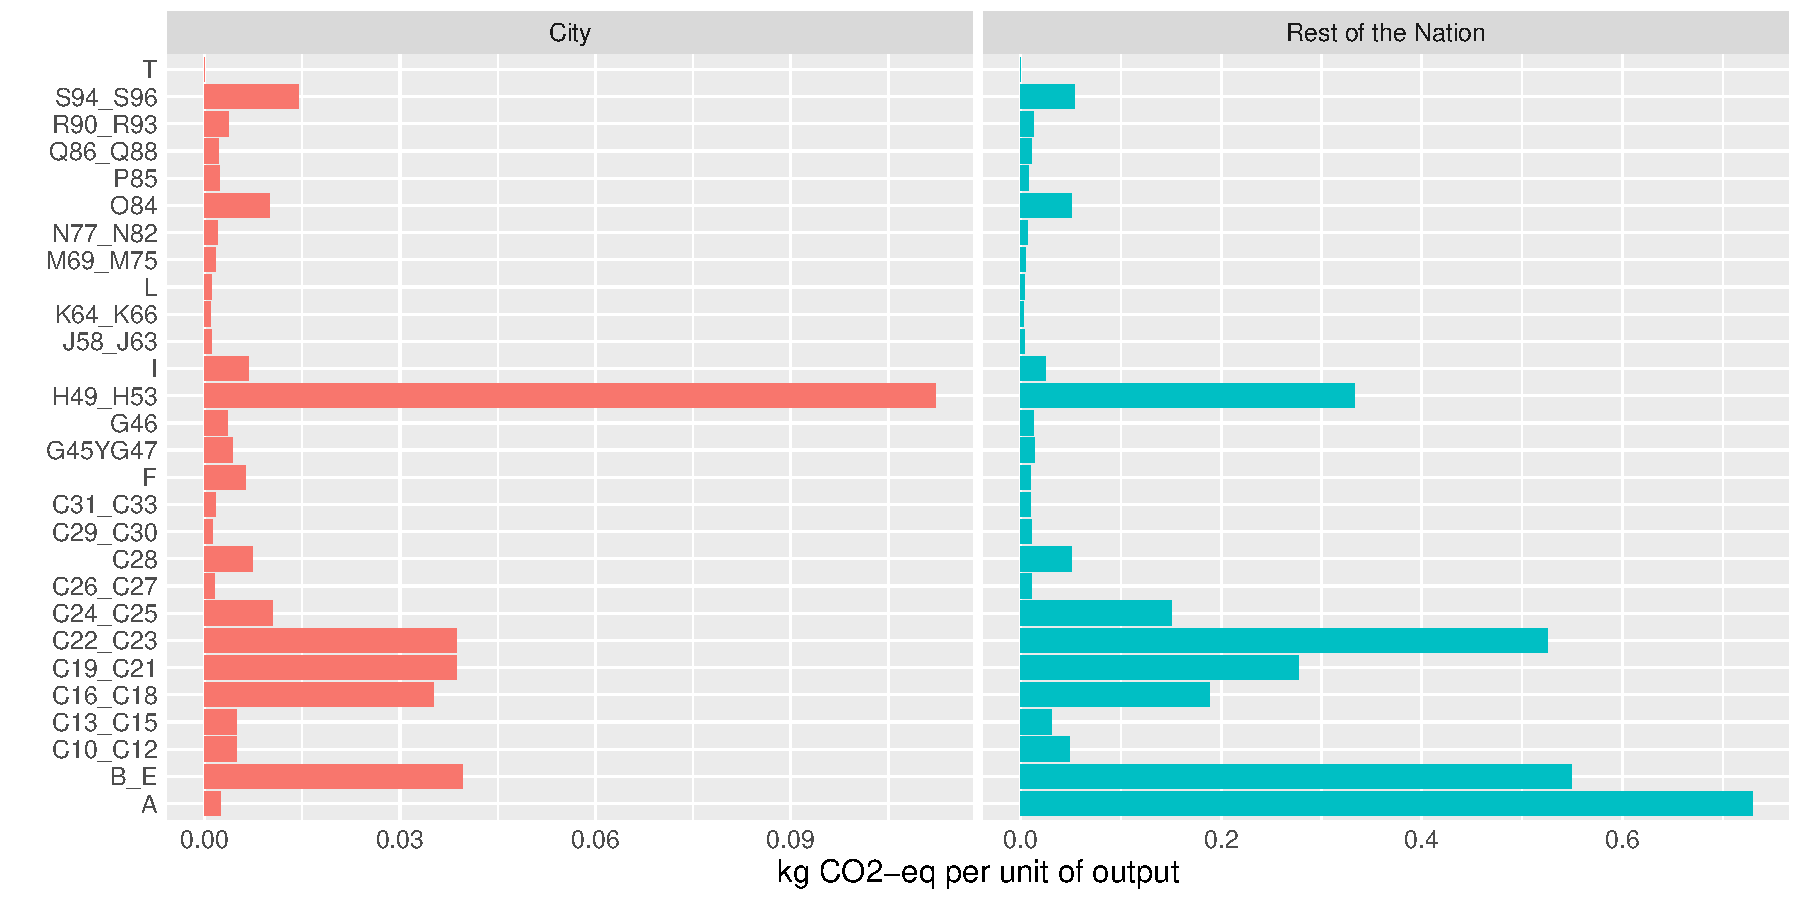
\includegraphics{graphics/intensity_ratios_2021.pdf}

}

\caption{\label{fig-intensity-ratio}Emissions factors by industry (NACE
rev.2) for the city and the rest of the nation, 2021. \emph{Source}:
Authors' calculations based on Eurostat's, FIGARO, and regional and city
accounts data}

\end{figure*}%

To address these challenges, we start from the excellent city AEI
released publically by the local administration for the period 1999-2021
\citep{am_inventario_2021}. The city's inventory reports all the
kilotonnes of \(\text{CO}_2e\) emissions that occur within the limits of
the city according to the Selected Nomenclature for Air Pollution (SNAP)
sector classification, with the exception of SNAP 01 as no emissions of
this type are found. It reports the same GHGs as Eurostat, with the
exception of \(NF_3\), for which there are no readings within the city
limits. It follows the EMEP/CORINAIR methodology to estimate total
atmospheric emissions, which causes small discrepancies with the IPCC
methodology.

We address these issues by following an inventory-first approach based
on imputation and secondary information
\citep{eurostat_manual_2015, corcoles_carbon_2024, sanchezserranoHuellaCarbonoHogares2023}.
Firstly, we assume that changing from the territorial to the residence
principle is possible using the share of the national bridge items on
the national inventory total provided by Eurostat for land and water
transport. For air transport we rely on data from
\citet{aena_estadisticas_2023} on airport operations. We allocate the
share of Madrid's Barajas Airport over the national emissions balance
from air travel, 18\% in 2021, to the sector of other transport (SNAP
08) in the city's inventory. Similarly, I assign 125.9\% of the balance
of land transport (a rather small quantity) to road transport (SNAP 07).
Hence, changing from one to another classification upscales the GHG
total, excluding households direct emissions, from 6356
\(\text{ktCO}_2e\) to 8001.7 \(\text{ktCO}_2e\) in 2021. Nevertheless,
we regard this as a conservative estimation, since, from a National
Accounts perspective, the emissions produced by many transport firms
from the rest of the country should be considered part of the city's
direct emissions. Due to lack of appropriate information, we do not
pursue additional residence-principle adjustments.

Secondly, we exploit the information in Annex I of Eurostat's Manual for
AEAs \citep{eurostat_manual_2015} to create a correspondence map between
SNAP and NACE (rev.2). Unfortunately, it is not a one-to-one matching
across classifications, so we rely on national data to derive a two-step
bridge matrix to move from the 10-sector SNAP classification, in which
the city inventory is presented, to the CRF/NFR classification used by
national AEIs and, finally, to the 28-industry NACE classification to
which the FIGARO GMRIO database has been aggregated to fit the estimated
city IOTs. We construct two matrices \(\textbf{S}\) and \(\textbf{N}\)
to achieve this transformation. The first one attaches to the CRF/NFR
classification the corresponding national GHG totals from Eurostat's
AEIs by source sector. Since there is a many-to-many relationship
between the two classifications we distribute each AEI sector's total as
a proportion on the SNAP row-sums total. In other words, we distribute
each CRF/NFR total \emph{proportionally} to the share of each total on
the SNAP cross-CRF/NFR total. This way, we proxy the missing
distributional information by the relative weight of each CRF/NFR code
falling within individual SNAP categories. The resulting \(s \times m\)
matrix \(\textbf{S}\), where \(s\) is the number of SNAP codes and \(m\)
the corresponding CFR/NFR codes, is normalized by the SNAP row sum
totals. The second matrix follows a similar procedure in which
Eurostat's national industry totals from the AEA are proportionally
distributed across CRF/NFR codes. We exclude households (HH\_TRA,
HH\_HEAT, HH\_OTH) from the list of NACE industries considered. The
\(m \times n\) matrix \(\textbf{N}^t\) is normalized by the row totals
of the corresponding CRF/NFR sectors. Using the city's inventory
\(e^{S}_{c}\), we derive the 28 NACE (rev.2) activities comprissing the
city \(\text{CO}_2e\) emissions accounts \(e^{N}_c\) as follows,
\vspace{-3pt}
\begin{equation}\phantomsection\label{eq-bridge-accounts}{ \textbf{e}^{N} = \textbf{e}^{S}\textbf{S}\textbf{N}^t }\end{equation}

Thirdly, we introduce a series of modifications to
\(\textbf{S}\textbf{N}^t\) to accommodate the peculiarities of the
city's economy. We redistribute 30\% the use of solvents and other
products (SNAP 06) to other direct emissions by households (HH\_OTH),
downscale Agriculture (A01-A03) to 10\% of the national proportion for
each SNAP sector, and eliminate all mining activity (B) altogether on
the premise that it does not exist or it is negligible. Most
importantly, we apply a reduction of 95\% in the amounts produced by the
electricity, gas, steam and air conditioning supply industry (D35),
which together with mining (B), water collection, treatment and supply
(E37) and sewerage, waste management, and remediation activities
(E37-E39) make up the total of the composite industry of mining and
supplies (B\_E). After these modifications, we allocate proportionally
the gap across the remaining industries to match the aggregate
constraints.

The resulting city accounts match the corrected inventory totals by
construction. We apply one additional correction to the intensities to
upscale (downscale) those sectors which are underrepresented
(overrepresented) in the city vis-à-vis the country by applying the
ratio of the city to the rest of the nation's output shares. This causes
some redistribution from manufacturing to services, which we deem
reasonable given the service orientation of the city economy
\citep{amMadridEconomia20232023}. Figure \ref{fig-intensity-ratio}
compares the emissions factors for the city of Madrid and the rest of
Spain. We can see that the two economies present some differences in
both the distribution and the magnitude of the emissions per unit of
output. Regarding the later, the emissions intensity for the whole
economy was in 2021 of 0.112 and 0.015 kg of \(\text{CO}_2e\) per unit
of output for the rest of the nation and the city, respectively, which
shows that the differences in magnitude are well within the general
difference between the two economies. On the other hand, we observe a
rather low intensity of transportation (H49\_H53) and public
administration (O85), and within tiny proportions for other services.
Finaly, we subtract the city vector from the national one to derive the
rest of the nation's \(\text{CO}_2e\) industry emission quantities. At
this point, computing the emission intensity-ratios is trivially done by
dividing industry \(\text{CO}_2e\) emissions by the corresponding gross
output value (P1). Table 1 shows the totals broken down by direct
emissions component, industries and the original inventory total.

A full AEA, however, must include direct emissions produced by household
activities. Eurostat divides them into three categories: heating and
cooling activities (HH\_HEAT), transport activities (HH\_TRA), and other
emissions-producing activities (HH\_OTH). The first two can be derived
bottom-up from ES-HBS micro data. We estimate emissions from heating and
transport activities by combining total quantities of different energy
products with the appropriate emissions factors provided by MITECO
\citeyearpar{miteco_calculadora_2023}. There is no information to derive
cooling-related emissions, and we exclude electricity as it represents
scope-2 emissions that are included in the corresponding energy
producing industry. An additional issue is that total direct transport
emissions by households are larger than all the transport emissions
reported in the city inventory. Besides the unlikely possibility that
households build fuel stocks, this is likely due to household members
driving to work outside the city limits. Since the latter uses direct
measurements from road transport, we decide to exclude 30\% of
households direct transport emissions in order to substract households'
road transport emissions from those made by firms and recorded in the
inventory (SNAP 07). This, again, produces some redistribution before
applying Equation~\ref{eq-carbon-footprint}. However, since the
residence principle rules the construction of the accounts, this missing
30\% from households direct emissions is kept for the purpose of
reporting direct transport emissions by households; we found no
reasonable criterion to substract the emissions from non-residents.
Lastly, we reallocate 30\% of total solvents and other products
emissions (SNAP 06) from the city's inventory to other direct emissions
by households. Table 1 shows the \(\text{CO}_2e\) total derived by
household activities (heating/cooling, transport, other) and by economic
activity across industries; we include the original AEI total reported
by the City Council for reference.

\begin{table}[!h]
\centering\begingroup\fontsize{9}{10}\selectfont
\begin{tabular}[t]{cccccc}
\toprule
Year & Heating & Transport & Other & Industries & Inventory\\
\midrule
2010 & 1335.7 & 4139.2 & 375.4 & 5825.7 & 8899\\
2011 & 1385.5 & 3981.7 & 369.4 & 5295.4 & 8261\\
2012 & 2139.5 & 3426.1 & 364.3 & 4676.1 & 8043\\
2013 & 1357.4 & 3152.5 & 362.7 & 5386.0 & 7802\\
2014 & 1279.9 & 2951.3 & 360.8 & 5395.2 & 7441\\
2015 & 1529.2 & 3069.0 & 211.2 & 5157.4 & 7187\\
2016 & 1190.8 & 2930.1 & 208.2 & 5879.9 & 7429\\
2017 & 1301.3 & 2925.9 & 166.4 & 5645.3 & 7219\\
2018 & 2025.1 & 2986.1 & 128.7 & 5222.1 & 7501\\
2019 & 1424.3 & 3045.6 & 126.3 & 5720.3 & 7230\\
2020 & 1779.6 & 1820.5 & 108.0 & 3470.3 & 5880\\
2021 & 1593.9 & 2312.2 & 109.3 & 3986.2 & 6356\\
\bottomrule
\end{tabular}
\endgroup{}
\caption{Breakdown of household direct emissions by type of activity, city industry emissions total, and the original city GHG inventory total, expressed in $\text{ktCO}_2e$. \textit{Source}: Authors’ own calculations.\label{tab:total-emissions}}
\end{table}

\subsection{Structural decomposition as a base for simulating trade
shocks on total emissions growth}\label{sec-subsec-decomposition}

In Section~\ref{sec-decomposition-simulation}, we use structural
decomposition analysis (SDA) to disentangle the contribution by changes
in emissions intensity, trade, technology, and final demand to the
variation in industry-level emissions for the input-output model in
equation \ref{eq-carbon-footprint}. SDA methodology uses the main
elements of the standard input-output model, such as the Leontief
inverse and the final demand vector, to decompose the change in one
variable into the changes of its constituent parts
\citep{artoDriversGrowthGlobal2014}. The application of SDA to the
quantification of the underlying sources of changes in \(\text{CO}_2e\)
emissions has grown considerably in the last decade from Dietzenbacher
and Los' seminal paper
\citeyearpar{dietzenbacherStructuralDecompositionTechniques1998}. More
recently, papers by \citet{hoekstra_emission_2016},
\citet{artoDriversGrowthGlobal2014}, and
\citet{xuStructuralDecompositionAnalysis2014} have expanded on the
original model to include additional decompositions to the the Leontief
inverse and final demand vector to capture specific effects, such as
separating trade and technology contributions, or distinguishing between
the level and composition impacts of final demand. In this paper, SDA
will allow us to break down the evolution of Madrid's consumption-based
CF into the contribution of emissions intensities, consumption, trade,
and technology. It must be noted that due to data limitations, the
decomposition uses flows at current prices.

For this purpose, we introduce a few modifications to the canonical
threefold decomposition in \citet[sec.~13.1.5]{miller_input-output_2022}
or \citet{dietzenbacherStructuralDecompositionTechniques1998}. We start
by defining \(\Delta \varepsilon\) as the growth in the volume of
\(\text{CO}_2e\) emissions between two periods, with superscripts \(0\)
and \(1\) for the two different years, which in this case are 2010 and
2021. By definition, \(\Delta \varepsilon\) is the result of our
standard model in the two periods as follows, \vspace{-3pt}
\begin{equation}\phantomsection\label{eq-varepsilon}{
\begin{aligned}
\Delta \varepsilon &= \varepsilon^1 -\varepsilon^0=\mathbf{e}^1\mathbf{L}^1\hat{\mathbf{y}}^1 - \mathbf{e}^0\mathbf{L}^0\hat{\mathbf{y}}^0
\end{aligned}
}\end{equation} where \(\mathbf{e}\), \(\mathbf{L}\),
\(\hat{\mathbf{y}}\) are the \(1 \times n\) \(\text{CO}_2e\) emissions
intensity vector, the Leontief inverse, and the \(n \times n\)
diagonalized vector of final household consumption, respectively. From
equation \ref{eq-varepsilon} we can follow the standard SDA methodology
\citep[sec.~13.1.1 to
13.1.5]{dietzenbacherStructuralDecompositionTechniques1998, miller_input-output_2022}
to expand and rearrange the definition of \(\Delta \varepsilon\) and
break it down into the three components of the basic additive
decomposition. As noted by
\citet[p.~310]{dietzenbacherStructuralDecompositionTechniques1998},
structural decompositions are non-unique, but taking the average of the
two polar decompositions provides a sufficient approximation to the
average of all possible approaches. Equation~\ref{eq-sda-basic} presents
the threefold decomposition described by
\citet[13.1.5]{miller_input-output_2022}, which presents separately the
effects of changes in emissions intensity, the technique of production,
and final consumption demand, which add up to \(\Delta \varepsilon\) by
construction. \vspace{-3pt}
\begin{equation}\phantomsection\label{eq-sda-basic}{
\begin{aligned}
\Delta \varepsilon&= \frac{1}{2}\underbrace{(\Delta \hat{\mathbf{e}})(\mathbf{L}^0\hat{\mathbf{y}}^0 + \mathbf{L}^1\hat{\mathbf{y}}^1)}_{\text{emissions intensity change}} \\ 
& + \frac{1}{2}\underbrace{\lbrack\hat{\mathbf{e}}^0(\Delta \mathbf{L})\hat{\mathbf{y}}^1 + \hat{\mathbf{e}}^1(\Delta \mathbf{L})\hat{\mathbf{y}}^0\rbrack}_{\text{technological change}} \\
& + \frac{1}{2}\underbrace{(\hat{\mathbf{e}}^0\mathbf{L}^0 + \hat{\mathbf{e}}^1\mathbf{L}^1)(\Delta \hat{\mathbf{y}})}_{\text{final consumption change}}
\end{aligned}
}\end{equation} However, the Leontief inverse captures and, thus, blurs
differences in trade and technology. To tell the contributions from
trade and technology apart, we draw from the decomposition within a
multiregional framework of the \(\mathbf{A}\) matrix into the Hadamard
product of two component matrices, \(\mathbf{C} \otimes \mathbf{H}\), as
described in detail in \citet{xuStructuralDecompositionAnalysis2014},
\citet{artoDriversGrowthGlobal2014}, and \citet{hoekstra_emission_2016}.
In this setting, matrix \(\mathbf{H}\) contains the total intermediate
input requirements irrespective of the source country, such that
\(z_{ij}^{s}=\sum_r z_{ij}^{rs}\), as described in
\citet{hoekstra_emission_2016}. Conversely, matrix \(\mathbf{C}\)
contains the share of all inputs of good \(i\) from country \(s\) coming
from country \(r\), where the corresponding elements are derived as
\(c_{ij}=a_{ij}^{sr}/h_{ij}^r\).

Starting from \(\mathbf{L}=(I - \mathbf{C} \otimes \mathbf{H})^{-1}\),
\citet[p.~607]{miller_input-output_2022} show that
\(\Delta \mathbf{L} = \mathbf{L}^1(\Delta \mathbf{C}\mathbf{H})\mathbf{L}^0\),
where \(\Delta \mathbf{C}\mathbf{H}\) can be itself divided into the
specific \(\Delta \mathbf{C}\) and \(\Delta \mathbf{H}\) effects,
\vspace{-3pt} \[
\Delta \mathbf{C}\mathbf{H}=\frac{1}{2}(\Delta \mathbf{C})(\mathbf{H}^0 + \mathbf{H}^1) + \frac{1}{2}(\mathbf{C}^0 + \mathbf{C}^1)(\Delta \mathbf{H})
\] Using this useful decomposition, we we can piece all previous
elements together and split the technological change effect from
\ref{eq-sda-basic} into a trade and pure technique of production
contribution, so that we can rewrite the decomposition formula and reach
our final expression as follows \vspace{-3pt}
\begin{equation}\phantomsection\label{eq-str-decomp}{
\begin{aligned}
\Delta \varepsilon&= \frac{1}{2}\underbrace{(\Delta \hat{\mathbf{e}})(\mathbf{L}^0\hat{\mathbf{y}}^0 + \mathbf{L}^1\hat{\mathbf{y}}^1)}_{\text{emissions intensity change}} \\ 
%& + \frac{1}{2}\underbrace{\lbrack\hat{\mathbf{e}}^0(\Delta \mathbf{L})\hat{\mathbf{y}}^1 + \hat{\mathbf{e}}^1(\Delta \mathbf{L})\hat{\mathbf{y}}^0\rbrack}_{\text{technological change}} \\
& + \frac{1}{4}\underbrace{ \lbrace \hat{\mathbf{e}}^0 \mathbf{L}^0 \lbrack \Delta \mathbf{C} \otimes (\mathbf{H}^0 + \mathbf{H}^1)  \rbrack \mathbf{L}^1 \hat{\mathbf{y}}^1 \rbrace }_{\text{trade structure change}} \\
& + \frac{1}{4}\underbrace{ \lbrace \hat{\mathbf{e}}^0 \mathbf{L}^0 \lbrack (\mathbf{C}^0 + \mathbf{C}^1) \otimes \Delta \mathbf{H} \rbrack \mathbf{L}^1 \hat{\mathbf{y}}^1 \rbrace }_{\text{technological change}} \\
& + \frac{1}{2}\underbrace{(\hat{\mathbf{e}}^0\mathbf{L}^0 + \hat{\mathbf{e}}^1\mathbf{L}^1)(\Delta \hat{\mathbf{y}})}_{\text{final demand change}}
\end{aligned}
}\end{equation}

Splitting \(\mathbf{A}\) into the element-wise product of matrices
\(\mathbf{C} \otimes \mathbf{H}\) presents us with the opportunity to
simulate changes in trade patterns on the assumption that the technique
of production remains unaffected. In section
\ref{sec-decomposition-simulation}, after presenting the structural
decomposition results, we introduce a series of simulation results to
illustrate the potential effect of blunt decoupling or global supply
chain restructuring on total consumption emissions. The premise is that
substituting one supplier from another, even though these systemic
transformations are very hard to come by in practice, may have a
potentially beneficial or adverse contribution to decarbonization
efforts. Furthermore, by providing a transparent quantification of this
potential contribution we expect to facilitate the discussion about
prioritizing local drivers or global suppliers in implementing
decarbonization policies.

The overall approach consists in downscaling the participation of
decoupling countries on the global supply of inputs to industry \(j\)
and, conversely, upscaling the input coefficient of the remaining
industries by proportionally allocating the total amount of input value
that is no longer coming from decoupling countries. We introduce this
changes in matrix \(\mathbf{C}\), which we then use to retrieve matrix
\(\mathbf{A}\) and \(\mathbf{L}\), such that \vspace{-3pt} \[
\mathbf{A}^{new}=\mathbf{C}^{new} \otimes \mathbf{H}^{old}
\] From this point we simply follow the standard approach from section
\ref{sec-method} to derive the new emissions level and distribution.

\section{Results}\label{sec-results}

\subsection{Industry drivers and suppliers of the city's GDP
CF}\label{sec-subsec-results-gdp}

We estimate the total CF of the city's gross domestic product (GDP) in
2021 to be in the order of 17447 \(\text{ktCO}_2e\), from which 2699
\(\text{ktCO}_2e\) are direct \(\text{CO}_2e\) emissions generated
within the city limits. This is 62.4\% of the emissions estimated for
2010, when the total CF of domestic activity was 27963
\(\text{ktCO}_2e\), of which 3567 \(\text{ktCO}_2e\) resulted from
direct emissions. In 2021, 15\% of emissions came from the city, whereas
the rest of the nation and the rest of the world contributed by 33\% and
51\%, respectively. Conversely, in 2010, the rest of the world accounted
for 47\% and the rest of the nation for 40\% of total emissions. We
observe a decline in total emissions but an increased relevance of the
global supply, as the rest of the world captures a substantially larger
share of scope-3 emissions.

Figure~\ref{fig-cf-growth-period} shows the time series of emissions
volume by source area from 2010 to 2021. To zoom in on the underlying
trends, the European Union, the United States, and China have been
separated from the rest of the world's total. In general we observe a
decline for all source areas in accordance with a declining total.
Nevertheless, across the period we observe a redistribution of emissions
from China to the United States after a period reversal from 2014 to
2018. The ratio of total emissions coming from China to those from the
United States went down from 2.68 to 2.07, which amounts to 338.6
\(\text{ktCO}_2e\). This concentrates on mining and energy supply
(B\_E), whose emissions declined for China but shot up for the United
States. The same tendency can also be observed for other sectors such as
manufacturing of chemicals, coke and petroleum products (C19\_C21),
manufacture of other machinery and equipment (C\_28) or wholesale and
retail trade (G45YG47). In the case of mining and energy supply, imports
from China fell slightly whereas those of the United States went up from
22.17 to 86.35 million euros. Nonetheless, looking at emissions factors,
we can observe that there are similar improvements in efficiency in
China versus the US for mining and energy supply, whereas for other
equipment or trade the efficiency gains almost double the ones realized
in the US or Germany. Hence, even with expanding demand for
manufactures, the relative and absolute decline is noticeable in the
time series.

\begin{figure}[!ht]

\centering{

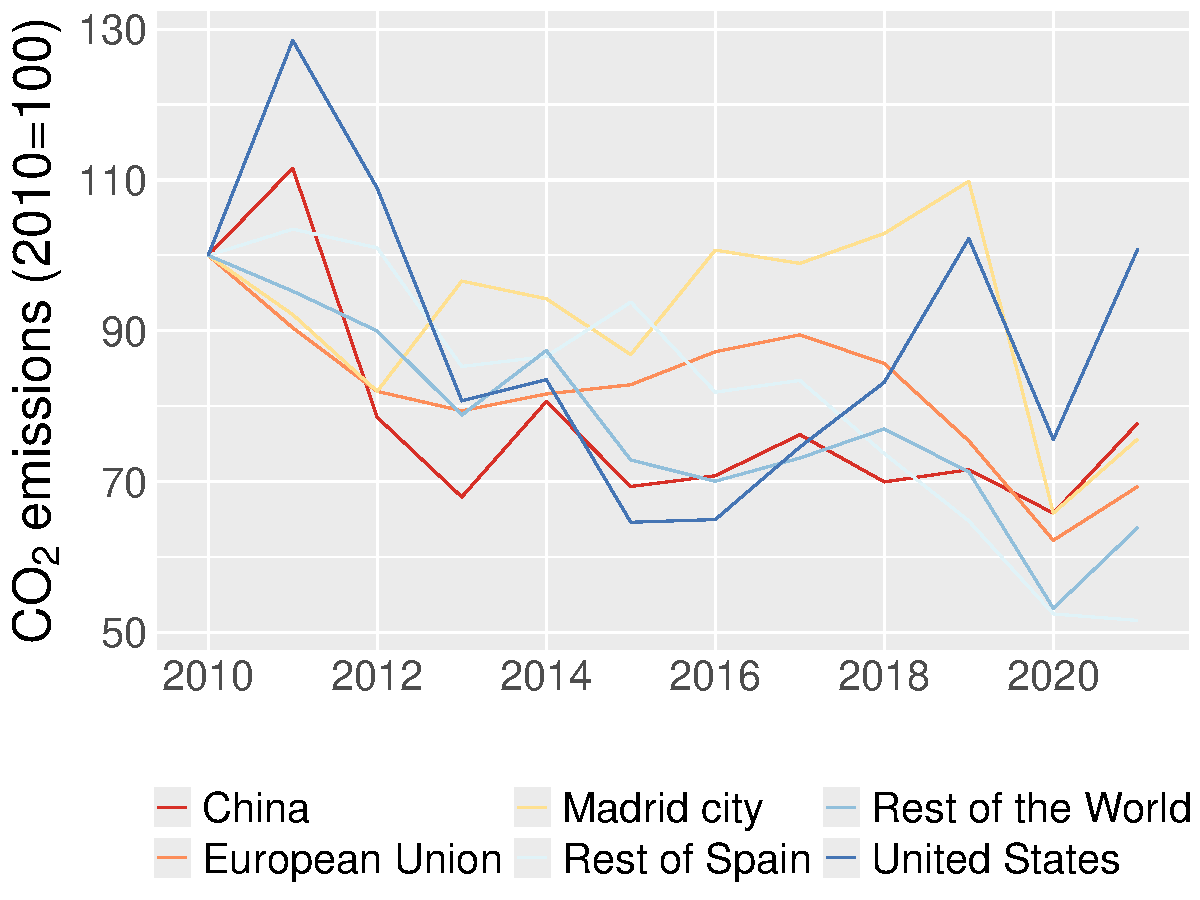
\includegraphics{graphics/emisiones_crecimiento_por_pais_2021.pdf}

}

\caption{\label{fig-cf-growth-period}Decomposition of \(\text{ktCO}_2e\)
emissions growth by main geographical area, 2010-2021 (2010=100).
\emph{Source}: Authors' own calculations}

\end{figure}%%
\begin{figure}

\centering{

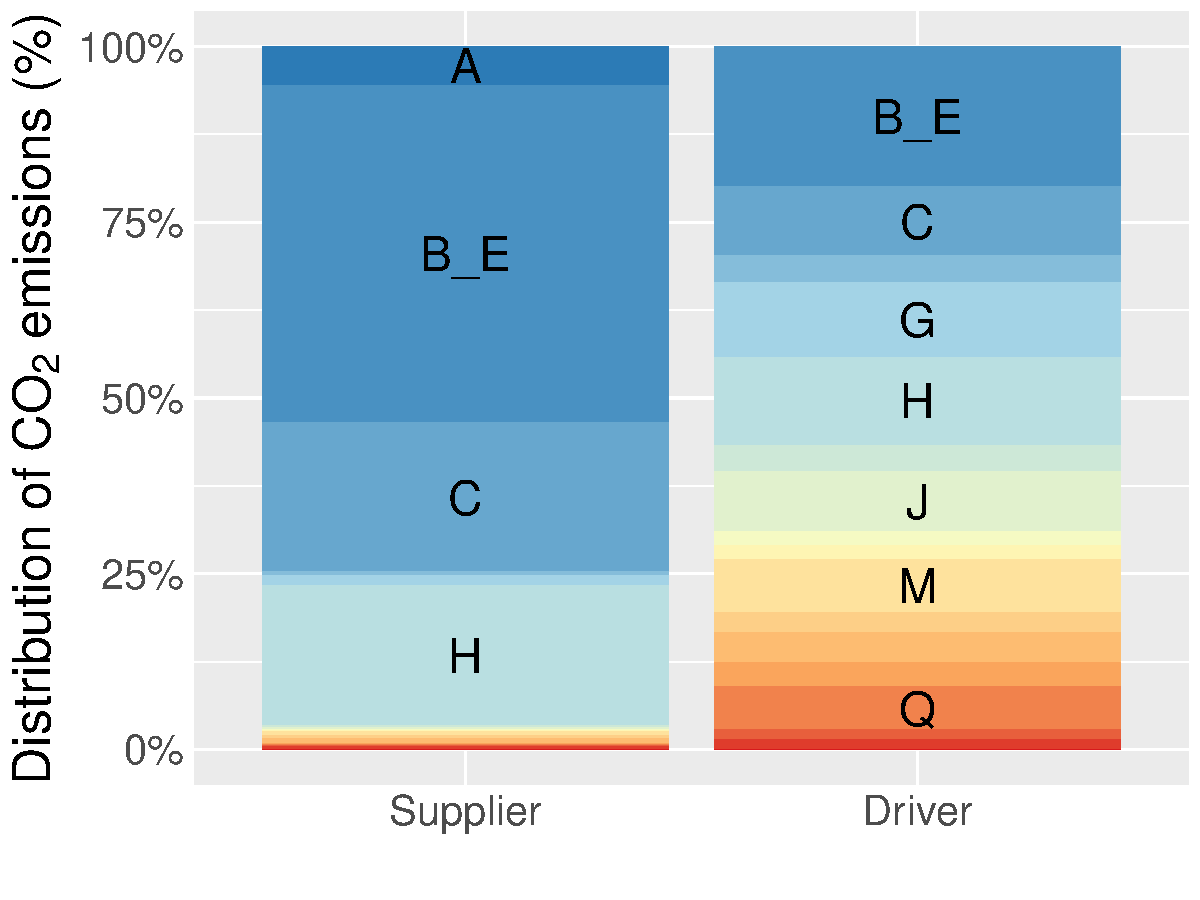
\includegraphics{graphics/emisiones_pie_chart_2021.pdf}

}

\caption{\label{fig-cf-supplier-driver}Distribution of
\(\text{ktCO}_2e\) emissions by supplier and driver sector, 2021.
\emph{Note}: only sectors contributing in more than 5\% are labeled in
the plot. \emph{Source}: Authors' own calculations}

\end{figure}%%
\begin{figure}

\centering{

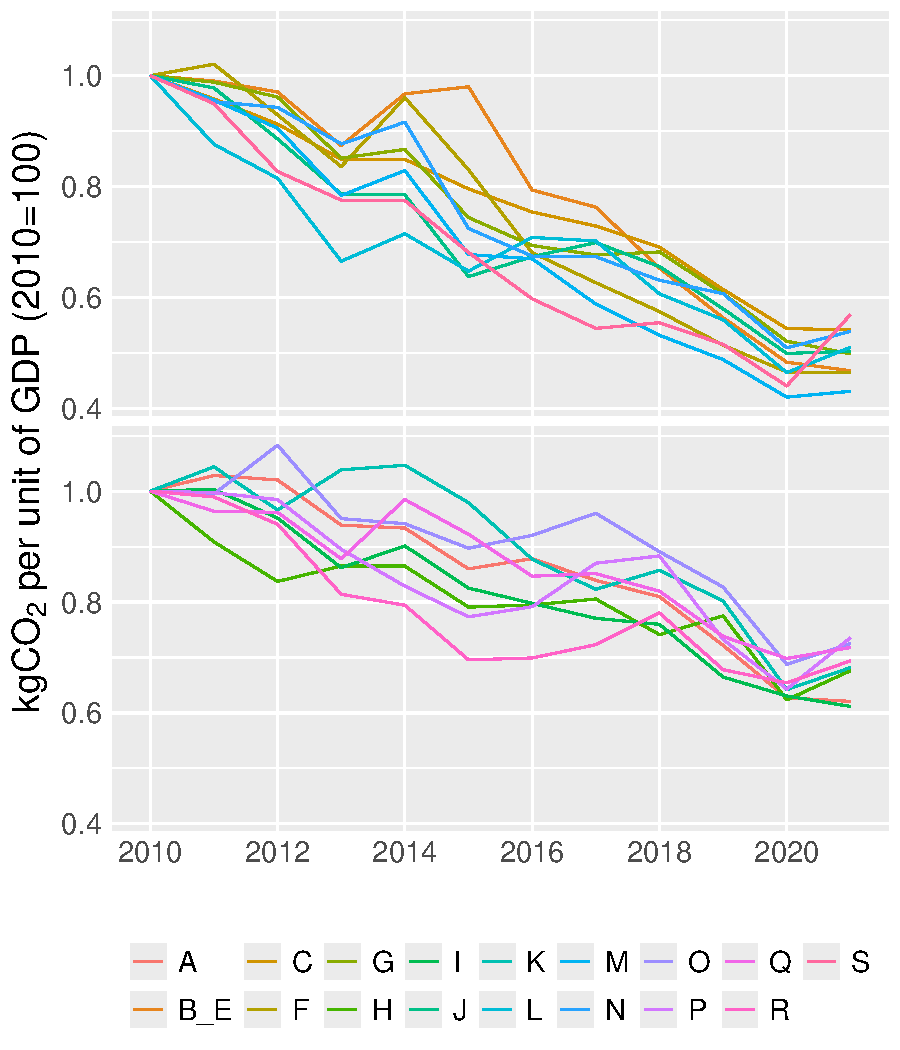
\includegraphics{graphics/factores_crecimiento_por_sector_2021.pdf}

}

\caption{\label{fig-cf-growth-factors}Evolution of total
\(\text{kgCO}_2e\) per unit of city GDP, 2010-2021 (2010=100).
\emph{Source}: Authors' own calculations}

\end{figure}%

In the same way that upstream emissions come predomintly from energy and
transportation industries, learning about the sectors driving indirect
emissions presents the responsibilities in a clear way. Incidentaly,
this enhences the ability to target the correct industries for
environmental policies at city scale.
Figure~\ref{fig-cf-supplier-driver} aggregates the contribution of
2-digit industries as suppliers and drivers of emissions by aggregating
the row or column totals from the CF matrix in equation
\ref{eq-carbon-footprint}, respectively. The first bar indicates that
three sectors: mining and energy products (B\_E), manufacturing (C), and
transportation and storage (H), account for more than 90\% of total
emissions embedded on goods and services imported by domestic
expenditures. Conversely, from the standpoint of the city's final
demand, we see that sector responsibility is more balanced, even if the
same sectors together with wholesale and retail trade (G) trigger 50\%
of total city emissions.

Looking at the driver industries of the city's CF, figure
\ref{fig-cf-sector-source} shows the two-dimensional distribution of the
total CF of the city broken down by industry and main source area. The
first thing to notice is the strong discrepancy between direct and
indirect emissions, but also how the gap behaves across industries. As
noted in figure \ref{fig-cf-supplier-driver}, the largest contributor is
the composite sector of mining and energy supply (B, E), which accounts
for 3477 \(\text{ktCO}_2e\). They come predominantly from the city, but
in 2021 1142 \(\text{ktCO}_2e\) were imported from the rest of Spain and
1789 \(\text{ktCO}_2e\) from the rest of the world. The situation
changes for other industries. The second largest driver is the wholesale
and retail industry (G), in which the rest of Spain dominates with 50\%
of the total. An even larger 71\% share is obtained for transportation
and storage, but the picture holds for most sectors. This highlights how
urban economies are crucially integrated within larger metropolitan or
country-spanning economic agglomerations.

\begin{figure*}[!ht]

\centering{

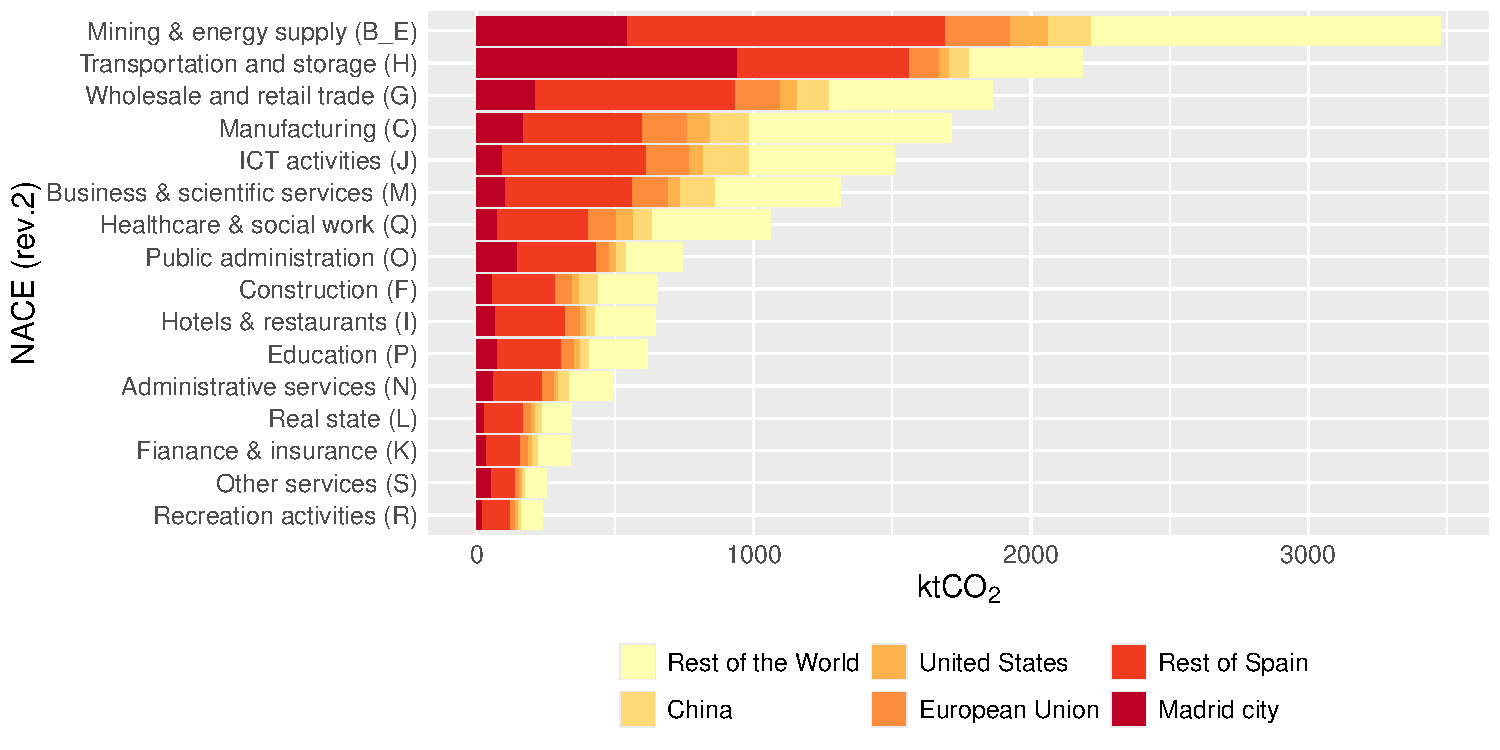
\includegraphics[width=1\textwidth,height=\textheight]{graphics/emisiones_gdp_madrid_area_industry_ES30_2021.pdf}

}

\caption{\label{fig-cf-sector-source}Total embedded GDP-linked emissions
from Madrid by sector and geographical origin, 2021. \emph{Note}:
Agriculture (A) and Household activities (T) are excluded due to very
low amounts. \emph{Source}: Authors' own calculations}

\end{figure*}%

Interestingly for Madrid, the industry of ICT activities (J), which is
one of the main growth engines and vectors of specialization of the city
economy, has a relatively large scope-3 CF. This works as a cautionary
tale about the need to include upstream emissions to properly evaluate
the environmental standing of service-driven growth. If the domestic
footprint of the industry reaches a relatively modest 94
\(\text{ktCO}_2e\), the direct plus indirect emissions total reaches
1507 \(\text{ktCO}_2e\). The same can be said of other economic bulwarks
such as business and scientific activities (M) or hotels and restaurants
(I).

In terms of \(\text{kgCO}_2e\) per unit of gross domestic product, the
highest intensity 0.736 in 2021 was in education (P), while the lowest
0.431 corresponds to business and scientific activities (M). Below 0.8
we find construction (F), real state (L), administration (N), and ICT
activities (J), with mining and energy supply (B\_E) at 0.468. Despite
the almost negligible contribution to GDP, agriculture (A) has a
medium-high intensity of 0.621, and hotels and restaurants (I),
transportation and storage (H), and recreation activities (R) show the
highest intensity ratios after education with 0.612, 0.676, and 0.694,
respectively. Manufacturing, on the other hand, has a mid-tier intensity
of 0.541, very similar to other services (S) 0.569. Whereas we can
expect high \(\text{ktCO}_2e\) services, e.g.~industries catering to
recreational demand or business activities, to be driven mostly by
robust final demand, the reality is that they are among the most
\(\text{CO}_2e\) intensive as well.

As per their evolution across the period,
Figure~\ref{fig-cf-growth-factors} shows the evolution of the direct
plus indirect carbon intensity of all 2-digit industries. We can
separate the ones displaying a stronger from a weaker downward trend in
\(\text{CO}_2e\) intensity. Despite accounting for the majority of
upstream emissions, the total intensity of mining and energy supply
(B\_E) and trade (G) have declined by -53.2\% and -50.2\%, respectively.
Business and scientific activities (M) show the best progress, with a
total -56.9\% fall in their \(\text{CO}_2e\) intensity, whereas
manufacturing indicates a more internally heterogeneous evolution that
renders a comparatively weaker -45.9\%. At a more granular 3-digit
level, we observe the lowest efficiency gains in food manufacturing
(C10\_C12) at -41.5\% and the highest in plastic and non-metallic
manufacturing with -53.8\%. Conversely, the worst performing 2-digit
industries are education (P) and recreation activities (R) with a
-26.4\% and a -30.6\% reduction, respectively. A relevant case is
transport and storage (H), which accounts for 13\% of total emissions
but whose \(\text{CO}_2e\) intensity has declined comparatively less by
a -32.4\%. Overall, the tendency seems to have stalled across the board
in 2020, even reversing slightly for some industries, but we would need
to include more recent years to fully grasp any persistent change.

\subsection{\texorpdfstring{Households' contribution to total \(CO_2e\)
emissions from
Madrid}{Households' contribution to total CO\_2e emissions from Madrid}}\label{sec-subsec-results-households}

\begin{figure*}

\centering{

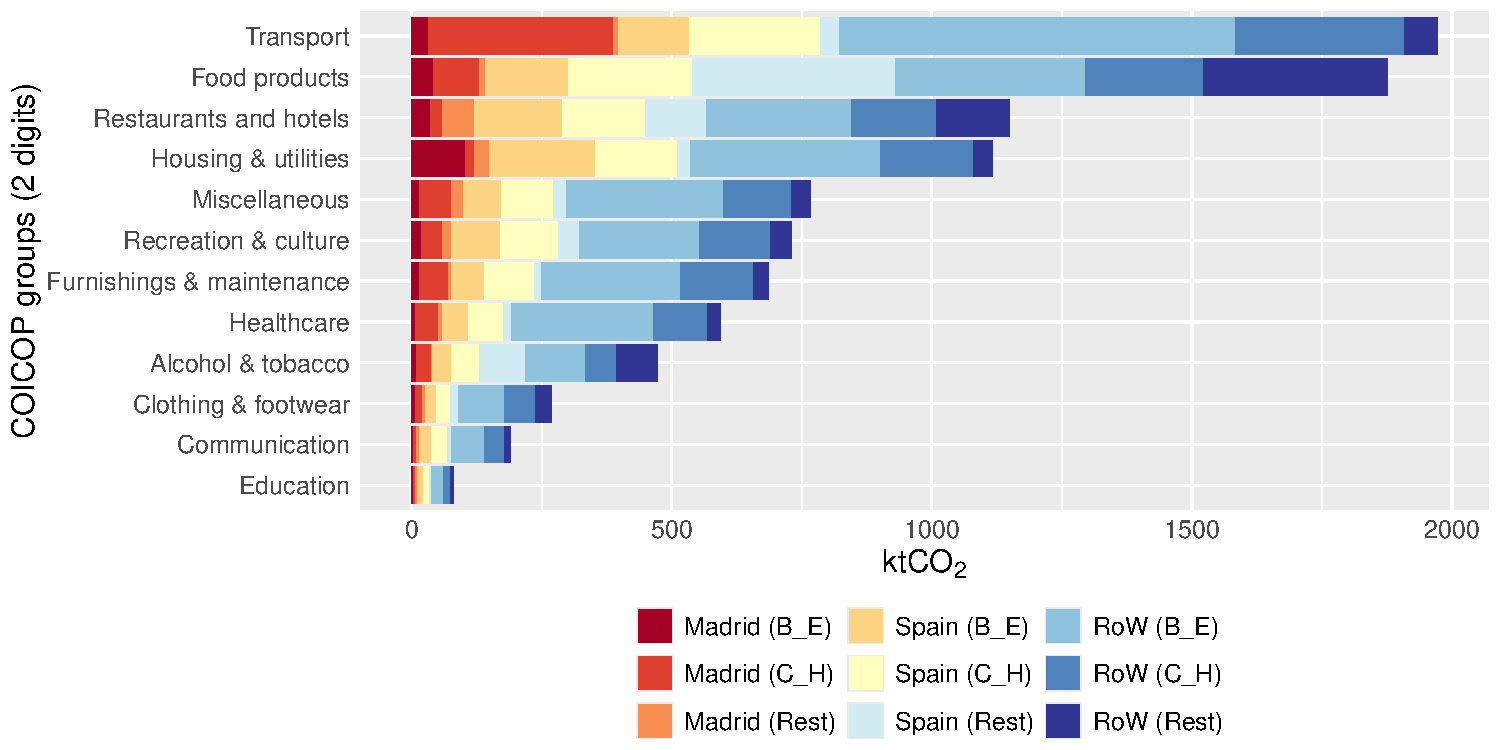
\includegraphics[width=1\textwidth,height=\textheight]{graphics/emisiones_coicop_nace_area_ES30_2021.pdf}

}

\caption{\label{fig-cf-consumption-source}Total embedded household
consumption-linked emissions from Madrid by driver consumption purpose
and supplier sector and geographical area, 2021. \emph{Note}:
Agriculture (A) and Household activities (T) are excluded due to very
low amounts. Whenever we make reference to (the rest of) Spain, we
exclude emissions and spending from Madrid. \emph{Source}: Authors' own
calculations}

\end{figure*}%

Despite a variety of challenges
\citep{macekuraMismeasureProgressEconomic2020, stiglitz_report_2009},
gross domestic product remains the go-to indicator of economic activity.
As such, it has allowed us to derive the total emissions which the
city's final demand is responsible for. This includes government
spending, net exports, and investment in addition to final consumption.
However, if we are interested in the environmental impact of material
well-being, we are forced to focus on households' final consumption
expenditure \citep{sala_consumption_2019}. In 2021, we estimate that the
CF of households in the city of Madrid totaled 13921 \(\text{ktCO}_2e\),
coming slightly down from 19424 \(\text{ktCO}_2e\) in 2010. From these,
4015 \(\text{ktCO}_2e\) or 28.8\% correspond to direct emissions by
households in 2021. Final consumption expenditure explains the other
9905 \(\text{ktCO}_2e\), which is equal to 0.163 \(\text{kgCO}_2e\) per
unit of nominal spending, which is in the low end of the urban density
distribution \citep{corcoles_carbon_2024, ivanova_mapping_2017}. In per
capita terms, the average resident emitted 4194 \(\text{kgCO}_2e\) in
2021 and 5908 \(\text{kgCO}_2e\) in 2010. As stated in equation
\ref{eq-carbon-footprint-households}, these figures combine the
emissions required from firms along the entire international supply
chain to cater to households' consumption needs and the emissions that
result from households' direct activities, primarily home temperature
regulation and private road transport.

Figure~\ref{fig-cf-consumption-source} shows the magnitude and
geographical distribution of the total emissions requirements for
meeting nominal consumption demand by main COICOP group in 2021. As
noted in section \ref{sec-method-household}, once we derive the vector
of industry \(\text{CO}_2e\) totals according to equation
\ref{eq-carbon-footprint}, we revert the procedure to go back from the
industry-based classification to COICOP and producer's prices so that we
can report industry totals by consumption purpose. Note, however, that
this totals \emph{exclude} direct emissions by households-qua-producers,
so that transportation \(\text{CO}_2e\) volumes belong exclusively to
services purchased by households and does not include, for instance, the
use of private cars. The first thing to notice in the chart is that
transportation is, in fact, at the top with 1972 \(\text{ktCO}_2e\).
Food products and housing and utilities follow closely at 1876
\(\text{ktCO}_2e\) and 1118 \(\text{ktCO}_2e\), respectively.
Accomodation, caterings, and restaurants, which represent an important
driver of economic activity in the city, stand high on the raking at
1149 \(\text{ktCO}_2e\). These four categories make up 61.7\% of total
consumption-linked emissions in Madrid. Education, clothing and
footwear, and communications generate the least emissions. Fron the
standpoint of the geographical distribution of emissions, the city's
weight is highest for transport, whereas the rest of Spain dominates in
restaurants, food products, and housing supplies. The rest of the world
is most important for transportation services, and very similar for food
and restaurants and hotels. Proportionally, its largest share is in
healthcare, although the emissions total is relatively low compared with
the top consumption groups.

Additionally, Figure~\ref{fig-cf-consumption-source} breaks down
emissions by three main composite supplying sectors: mining and energy
supply (B\_E), manufacturing and transport (C\_H), and all remaining
industries (Rest), such as agriculture, recreational services or
construction. In the same way that Figure~\ref{fig-cf-supplier-driver}
showed that the first two sectors dominate the upstream supply of
\(\text{CO}_2e\) emissions, Figure~\ref{fig-cf-consumption-source}
synthesizes the supply and driver perspective by accounting for the
geographical-sectoral supply distribution of \(\text{CO}_2e\)
requirements by consumption purpose. It indicates, for instance, that
approximately a third of the transport services' footprint comes from
the domestic transport industry, with a strong contribution from the
rest of the world and the rest of Spain. Food products have a
substantial component of embedded emissions from manufacturing and
transportation, and in general from the rest of the world, which
accounts for more than 50\% of the total. The same holds for
accommodation and restaurants, although the contribution from the rest
of Spain is in this case the most relevant. Recreation and culture has a
considerable indirect CF that is masked by its low direct emissions
volume. More importantly, this indirect footprint relies on a relatively
large upstream contribution by foreign manufacturing and transportation.
As indicated above, the largest contribution from the rest of the world
is in healthcare services and products, but we can see now that this is
mostly due to mining and energy supply. For clothing and footwear the
proportion of the foreign contribution is similar but the weight of
manufacturing is on a level with energy supply.

\begin{table}[!h]
\centering\begingroup\fontsize{8}{9}\selectfont
\begin{tabular}[t]{lcccc}
\toprule
Expenditure category & $\text{kgCO}_2e$/\euro{} & $\text{ktCO}_2e$ & \euro{M} & Growth \\
\midrule
01 Food products & 0.272 & 18.9 & 11.3 & -0.9\\
02 Alcohol \& tobacco & 0.287 & 4.8 & 2.7 & 0.3\\
03 Clothing \& footwear & 0.132 & 2.7 & 3.4 & -3.5\\
04 Housing \& utilities & 0.066 & 11.3 & 27.7 & -5.8\\
05 Furnishings & 0.195 & 6.9 & 5.8 & -5.8\\
06 Healthcare & 0.213 & 6.0 & 4.6 & -1.3\\
07 Transport & 0.308 & 19.9 & 10.5 & -1.6\\
08 Communication & 0.123 & 1.9 & 2.6 & -4.6\\
09 Recreation \& culture & 0.172 & 7.4 & 7.0 & -1.8\\
10 Education & 0.087 & 0.8 & 1.5 & -5.8\\
11 Restaurants \& Hotels & 0.137 & 11.6 & 13.8 & -3.5\\
12 Miscellaneous & 0.139 & 7.7 & 9.1 & -3.9\\
\bottomrule
\end{tabular}
\endgroup{}
\caption{$\text{kgCO}_2e$ per unit of nominal household spending ratios and descriptives in 2021. \textit{Note}: $\text{ktCO}_2e$ emissions and \euro{M} spending figures are presented in shares, whereas the last column shows the 2010-2021 period compound growth rate of the emissions ratios by expenditure category. \textit{Source}: Authors’ own calculations.\label{tab:spending-intensity}}
\end{table}

\begin{table*}[!ht]
\centering
\begin{tabular}[t]{lcccccccccc}
\toprule
Emissions group & Q1 & Q2 & Q3 & Q4 & Q5 & 15-34 & 35-54 & 55-70 & +71 & Total\\
\midrule
Equivalized income \euro{} & 17116 & 21784 & 25373 & 29045 & 36428 & 23057 & 25514 & 26633 & 27265 & 25931\\
Equivalized $\text{kgCO}_2e$ & 2318 & 3940 & 5246 & 7570 & 11234 & 5774 & 6333 & 6503 & 5046 & 6053\\
\addlinespace
01 Food products & 269 & 408 & 446 & 543 & 597 & 318 & 438 & 495 & 507 & 456\\
02 Alcohol \& tobacco & 61 & 149 & 221 & 225 & 333 & 140 & 186 & 265 & 165 & 200\\
03 Clothing \& footwear & 39 & 50 & 73 & 105 & 148 & 98 & 90 & 81 & 76 & 86\\
04 Housing \& utilities & 112 & 144 & 144 & 161 & 220 & 126 & 141 & 174 & 181 & 157\\
05 Furnishings & 32 & 46 & 83 & 153 & 249 & 100 & 89 & 129 & 190 & 118\\
06 Healthcare & 58 & 102 & 150 & 198 & 381 & 145 & 135 & 239 & 237 & 185\\
07 Transport & 140 & 280 & 463 & 716 & 1087 & 623 & 626 & 569 & 392 & 577\\
08 Communication & 41 & 55 & 58 & 64 & 70 & 52 & 54 & 62 & 68 & 58\\
09 Recreation \& culture & 35 & 57 & 86 & 128 & 274 & 95 & 132 & 139 & 87 & 124\\
10 Education & 16 & 29 & 59 & 76 & 193 & 19 & 108 & 79 & 46 & 95\\
11 Restaurants \& hotels & 81 & 168 & 332 & 448 & 984 & 375 & 493 & 461 & 329 & 450\\
12 Miscellaneous & 53 & 70 & 94 & 128 & 284 & 158 & 117 & 119 & 166 & 131\\
\addlinespace
Heating/cooling & 675 & 881 & 821 & 908 & 984 & 702 & 791 & 844 & 1070 & 859\\
Transport & 414 & 1147 & 1590 & 2430 & 2461 & 2397 & 1677 & 1744 & 1097 & 1682\\
Other & 19 & 29 & 40 & 56 & 96 & 43 & 50 & 51 & 44 & 48\\
\bottomrule
\end{tabular}
\caption{Breakdown of households' average $\text{kgCO}_2e$ footprint of 2-digit consumption purposes and domestic activities by spending quintile and age group in Madrid, 2021. \textit{Source}: Authors’ own calculations.\label{tab:emissions-demographic}}
\end{table*}

From Figure~\ref{fig-cf-consumption-source} we can learn that
consumption spending drives an extremely large volume of indirect
emissions. However, this depends on two parameters: the level of final
demand and the carbon intensity of each consumption purpose. To
understand this difference, we need to derive intensity ratios by
2-digit COICOP groups. Table 2 shows the emissions intensity per unit of
nominal household spending (\(\text{kgCO}_2e\)\euro{}) of main
expenditure groups, followed by the shares of each category on total
embedded emissions and consumption spending. The last column reports the
2010-2021 compound growth rate of the intensity ratios. We can see that
spending on transportation and storage is the most \(\text{CO}_2e\)
intense in the city, whereas housing and utilities is in the opposite
situation. The outstanding contribution of transport spending is
explained by its 10.5\% share on total household spending and an
intensity of 0.308 \(\text{kgCO}_2e\)\euro{}, which explains its leading
position in figure \ref{fig-cf-consumption-source}. Similarly, housing
and utilities is less carbon intense, but tops the ranking with 27.7\%
of total expenditure. Lastly, it is worth noting that all groups'
intensity ratios are declining, with the exception of alcohol and
tobacco, albeit at different speeds. While the housing and utilities
group has reduced its emissions intensity by -5.8\% per year, food
products and transport have realized much smaller efficiency gains at
-0.9\% and -1.6\%, respectively.

At a more granular level (3-digit COICOP), the picture is validated with
a few exceptions. For food products, for instance, we see that the
emission intensity is driven down by food (011), with an average
compound growth of -0.9\% and an average factor of 0.3. For alcoholic
beverages (021) we see a moderate -1\% decline, where the emission
intensity of tobacco (022) grew by 1.7\%, both with high ratios similar
to food and non-alcoholic beverages. Clothing (031) and footware (032),
on the other had, have low intensities that are also underwent a robust
process of decline. For instance, clothing reduced its intensity by a an
average -3.7\% from an already low 0.202 intesity in 2010. The largest
reductions are, basides actual and imputed rentals (041-042), in other
services (127: -5\%), postal services (081: -15\%), insurance (125:
-4.1\%), and housing tools and equipement (055: -10.6\%). Communications
equipment (082: -7.5\%), household utensils (054: -10.5\%) and textiles
(052: -4.6\%) have also strongly reduced their \(\text{CO}_2e\)
intensity. On the oposite end, medical products and equipment (061: 1\%)
and other recreational goods and services (092: 3\%) stand out as
growing more carbon intensive.

We noted in section \ref{sec-method-household} that it is possible to
retrieve household-level CFs. After deriving 3-digit intensity ratios,
we impute the estimated total CF per consumption purpose to each
household reported in ES-HBS \citep{ine_encuesta_2024}, whose
aggregation matches the figures reported before by construction. Using
information on energy products (measured in physical units) and on
emissions factors from MITECO \citep{miteco_calculadora_2023}, we can
also impute the estimated \emph{direct} CF of household activity
\citep{corcoles_carbon_2024}. The resulting micro data creates a
distributional perspective into the volume of emissions triggered by
household decisions. This is crucial to understand the drivers of a
city's footprint and, most importantly, to act on them without disregard
for the economic inequalities that could compromise mitigation
strategies. For instance, the average equivalized household income after
taxes and transfers was \euro 25931 in 2021, but this glosses over
substantial distributional differences that can go from \euro 17116 on
average for the bottom 20\% to \euro 36428 for the corresponding top
20\% of the equivalized spending distribution.\footnote{Household
  equivalized income accounts for differences in a household's size and
  composition to make individual incomes comparable across household
  types. It adjusts total household income using the modified OECD
  equivalence scale, where the first adult counts as 1, but the second
  and each subsequent person aged 14 and over only 0.5, 0.3 to each
  child aged under 14 \citep{deatonAnalysisHouseholdSurveys1997}} Each
spending quintile represents aproximatedly 288006 households, but an
unequal number of people ranging from 698865 (Q1) to 655229 (Q5). This
translates into quite different emissions profiles and overall levels of
inequality in each group's contribution to climate change.

Table 3 presents the breakdown of households' average annual equivalized
\(\text{kgCO}_2e\) emissions by spending quintile and four age groups
(15-34, 35-54, 55-65, +71). It also separates the contribution of
2-digit COICOP groups and direct \(\text{CO}_2e\) emissions. We include
the aggregate figures for comparison. Unless stated otherwise, all
values are equivalized and refer to 2021. Overall, we see a strong
correlation between income and emissions levels. For instance, the
bottom 20\% of the spending distribution emitted an average of 2299
\(\text{kgCO}_2e\) in 2021, whereas the top 20\% contributed with 4.8
times as much \(\text{kgCO}_2e\). However, this distributional gap is
due not only to level but compositional changes. On the one hand,
\(\text{kgCO}_2e\) for all consumption purposes and domestic activities
increases with households' equivalized disposable income. While
education and restaurants \& hotels are the emissions groups with the
largest quintile gap, housing \& utilities and communication are the
ones with the lowest. In accordance with the environmental expression of
Engel's Law
\citep{browningEngelLaw2018, levinsonEnvironmentalEngelCurves2015}, we
tend to see essentials on the lower end of the gap distribution. Food
purchases are 51.8\% higher for the second than the first quantile, but
they only grow by 46.4\% from the second to the fifth quantile,
indicating the marginally decreasing growth in expenditure and emissions
as a function of income levels. Hence, to observe such a large
distributional gap, other consumption purposes need to reverse the
relationship between expenditure and income that obtains for essentials.
This is especially the case of restaurants and hotels. Equivalized
emissions grow by 1113.4\% from the bottom to the top quintile.
Similarly, for transport, recreation and cultural activities, and
miscellanea we find gaps of 678.5\%, 688.2\%, 434.9\%, respectively.
Education is an interesting case, since related emissions are
comparatively low, but due to the remarkable spending gap, we are left
with a 1106.2\% increase across the quintile distribution. The aggregate
picture is, therefore, a mixture of opposing tendencies. It seems clear
that any policy targetting consumption needs to reckon with this radical
difference between essentials and other expenditure groups in designing
mitigation plan.

\begin{table*}[!ht]
\centering
\begin{tabular}[t]{lccccccccc}
\toprule
Emissions group & Female & Male & Primary & Secondary & Tertiary & Full & Partial & Renteer & Free user\\
\midrule
Equivalized income \euro{} & 24692 & 26792 & 18382 & 22082 & 30975 & 28351 & 29118 & 19010 & 26530\\
Equivalized $\text{kgCO}_2e$ & 5655 & 6330 & 3370 & 5577 & 7038 & 6055 & 7061 & 5145 & 5961\\
\addlinespace
01 Food products & 452 & 458 & 407 & 455 & 466 & 504 & 470 & 370 & 428\\
02 Alcohol \& tobacco & 188 & 207 & 216 & 215 & 184 & 220 & 196 & 165 & 249\\
03 Clothing \& footwear & 95 & 81 & 45 & 71 & 105 & 80 & 96 & 76 & 152\\
04 Housing \& utilities & 175 & 145 & 135 & 157 & 162 & 182 & 144 & 128 & 147\\
05 Furnishings & 120 & 117 & 104 & 95 & 139 & 154 & 118 & 58 & 116\\
06 Healthcare & 213 & 167 & 143 & 192 & 188 & 249 & 161 & 110 & 145\\
07 Transport & 584 & 573 & 241 & 551 & 640 & 540 & 616 & 607 & 440\\
08 Communication & 61 & 56 & 49 & 58 & 60 & 62 & 53 & 56 & 74\\
09 Recreation \& culture & 142 & 114 & 44 & 113 & 142 & 123 & 147 & 93 & 203\\
10 Education & 89 & 98 & 150 & 40 & 123 & 54 & 88 & 161 & 37\\
11 Restaurants \& hotels & 391 & 482 & 165 & 388 & 531 & 382 & 570 & 368 & 776\\
12 Miscellaneous & 155 & 116 & 85 & 108 & 160 & 143 & 102 & 139 & 146\\
\addlinespace
Heating/cooling & 980 & 777 & 769 & 862 & 875 & 944 & 835 & 757 & 632\\
Transport & 1594 & 1722 & 610 & 1555 & 1926 & 1680 & 1786 & 1538 & 1842\\
Other & 47 & 49 & 29 & 43 & 57 & 48 & 53 & 42 & 53\\
\bottomrule
\end{tabular}
\caption{Breakdown of households' average $\text{kgCO}_2e$ footprint of 2-digit consumption purposes and domestic activities by gender, main education level, and tenure status in Madrid, 2021. \textit{Source}: Authors’ own calculations.\label{tab:emissions-demographic}}
\end{table*}

Comparing emissions from expenditure and activities, we can calculate
that while the top quintile represents 35.3\% of total emissions, or
4881.7 \(\text{ktCO}_2e\), the bottom quintile generates only 8\%. This
amounts to a gap of no less than 3778.6 \(\text{ktCO}_2e\). The gap in
emissions derived from expenditure is 3043.8 \(\text{ktCO}_2e\) and in
emissions-generating activities 734.8 \(\text{ktCO}_2e\). The ratio of
the last to the first quantile is 5.1 for the former and 3.1 for the
latter. Emissions inequality is higher in consumption than in direct
activities, but in transport activities the ratio is 6.2. Differences in
heating/cooling emissions are minor (1.6), indicating that they are
compararively much more income-inelastic. In terms of equivalized
emissions, differences are stronger in heating/cooling and as much in
transport activities and other emissions.

Subsetting by socio-demographic groups, as shown in Tables 3 and 4, we
find a different reading. Looking across age groups for the household
reference person we find some differences, particularly in terms of
average equivalized \(\text{kgCO}_2e\) and for the cases of transport
expenditure and activity. The central age groups (35-54, 55-70) have
higher equivalized income, expenditure, and \(\text{kgCO}_2e\), than the
young (15-34) and the old (\(+71\)), but only to a limited extent. In
equivalized terms, households whose reference person is female or male
show only small variations, with the exception of transport, recreation
activities, and hotels and restaurants, as well as heating/cooling
emissions, where the former is responsable for a larger
\(\text{kgCO}_2e\) volume. The opposite is true in the case of direct
transport activity, where male reference person households generate more
\(\text{kgCO}_2e\). As for the highest education level achieved by the
reference person, the overlap with income is visible, and we have a
strong jump from primary to secondary and, then, to tertiary in terms of
income but more than proportionally in terms of \(\text{kgCO}_2e\),
growing by 109\%. By education level, we can observe the largest
differences in recreation \& culture, restaurants \& hotels, and
transport activity. As per tenure status, the sharpest variation obtains
between partial owner and renteer, in large part seemingly due to the
substantial income difference between the two demographics.

We can illustrate the relative importance of the expenditure
\emph{structure} in addition to the expenditure level. While moderation
of expenditure levels have a straightforward implications for
households' CF, variation in the spending composition as a function of
per capita spending can have a less obvious but sizeable impact
\citep{levinsonEnvironmentalEngelCurves2015}. A possible implication of
Engel's Law is the non-linear growth in total emissions
\citep{browningEngelLaw2018, levinsonEnvironmentalEngelCurves2015}. As
we have seen, essentials, such as food or transport, are relatively more
carbon intensive than other products. If we imposed a poorer consumption
structure, hence a higer share of spending on essentials, on the the
upper segment of the spending distribution, we might increase, rather
than reduce, the total amount of consumption-related \(\text{ktCO}_2e\)
if consumption levels remained the same for the whole distribution.
However, the opposite seems true. Imposing the median consumption
structure above the \(50^{th}\) percentile would amount to a reduction
of 3688.2 \(\text{ktCO}_2e\) (26.7\%) in 2021. For comparison, total
\(\text{CO}_2e\) emissions caused by food spending will slightly
increase by 14.8\%, whereas for housing and utilities they would remain
at the same level. On the other hand, emissions from transport services,
hotels and restaurants , and recreation and culture will decline
noticeably by 15.8\%, 13.6\%, and 15.6\%, respectively. By looking at
the rest of consumption purposes we can see that furnishings and home
maintenance, healthcare, and miscellanea are more important as we move
up in the spending distribution, but nowhere near the case of education,
whose emissions would be almost negligible compared to the rest of
consumption groups.

Conversely, we can also evaluate the potential of mobility policies
vis-à-vis expenditure policies by simulating the impact on total
\(\text{CO}_2e\) that interventions targeting either a substantial
limitation of private emissions-generating road transport or the
increasing adoption of electric vehicles could potentially have. Table 3
highlighted the outstanding contribution of private mobility choices to
the average household's CF in Madrid. In this sense, reductions in
private transport outweight any reasonable intervention on consumption
demand. To exemplify this point, Figure~\ref{fig-cf-coicopCO2b} reports
how many \(\text{ktCO}_2e\) would the city save if households reduced
50\% of their use of private vehicles cummulatively from the richest to
the poorest of the target bottom decile of the intervention. In orther
words, by simulating a 50\% adoption of carbon-neutral transport
activities by households in the ninth, or from the ninth to the eighth,
and so on, decile, we can illustrate the total \(\text{ktCO}_2e\)
savings.Within the top 10\%, 20\%, 30\%, and down to 80\% we randomly
sample with probability \(1/2\) a series of households from the set of
those with positive fuel spending records. We then eliminate completely
their transport emissions and derive the new totals. This assumes that
all household members either switch to other means of transportation
(public transit, cycling or walking) or turn to electric vehicles (EVs)
to meet their mobility needs.

\begin{figure}

\centering{

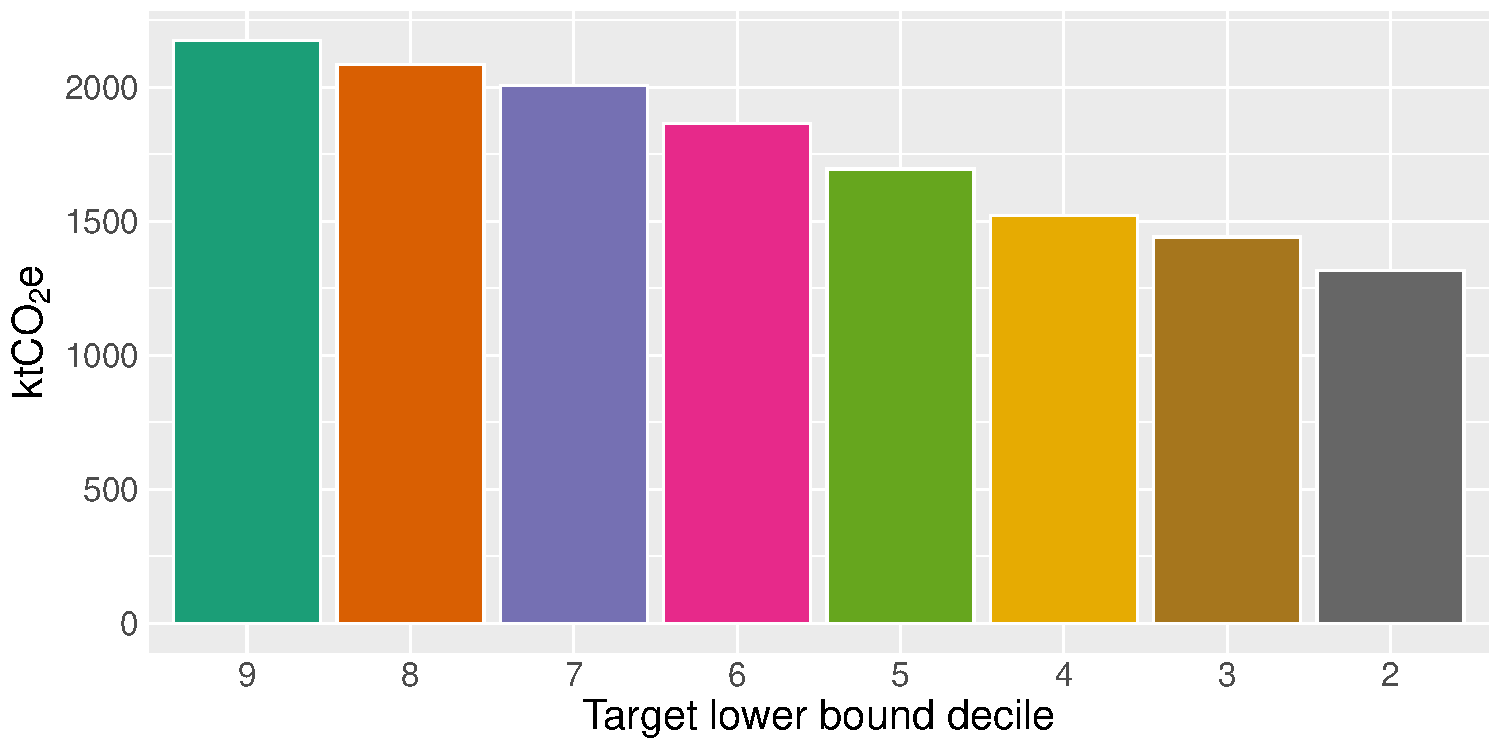
\includegraphics{graphics/simulation_evs_GHG_reduction.pdf}

}

\caption{\label{fig-cf-coicopCO2b}Simulated direct transport emissions
levels resulting from a 50\% addoption rate of carbon-free transport
activities by households from the top down to the corresponding bottom
spending decile of the intervention range, 2021. \emph{Source}: Authors'
own calculation.}

\end{figure}%

Figure~\ref{fig-cf-coicopCO2b} shows that the mitigation potential of
changes to private transport are considerable. Depending on the
penetration rate of (close to) carbon neutral means transportation
across the spending distribution, we obtain different \(\text{CO}_2e\)
savings. If we limit this transformation to the top 10\%, we find that
direct transport emissions by households go down from 2312.2
\(\text{ktCO}_2e\) to 2174.1 \(\text{ktCO}_2e\), which is a 6\%
reduction. Alternatively, if one in every two households implement this
drastic change, we would end up with 1694.9 \(\text{ktCO}_2e\), which
represents 26.7\% or 1694.9 \(\text{ktCO}_2e\) fewer direct transport
emissions. If this process reaches half of the household population, but
excluding the bottom 10\%, we would talk of approximately 43\% lower
direct transport emissions by households in 2021. By changing the
probability of adoption, we obtain very different emissions reduction
totals. With one out of every twenty households in the top 50\%
following suit, we get as little as a 3.4\% reduction. Conversely, if
the likelihood of adoption increases to 80\% among the top three
deciles, we could see direct transport emissions falling to 1702.8
\(\text{ktCO}_2e\), which is 26.4\% less. These scenarios highlight the
enormous potential for \(\text{CO}_2e\) emissions reduction that could
derive from a strong commitment to fostering the adoption of electric
vehicles, public transportation, or cycling.

\subsection{Breaking down the drivers of the carbon footptint's growth
path}\label{sec-decomposition-simulation}

Sections \ref{sec-subsec-results-gdp} and
\ref{sec-subsec-results-households} have reported the level,
composition, and evolution of 3-scope \(\text{CO}_2e\) emissions driven
by the city's gross domestic product and final household consumption.
Using structural decomposition analysis (SDA) we can now delve into the
underlying factors determining emissions generation. As presented in
section \ref{sec-subsec-decomposition}, we break total emissions down by
the contribution of intensity, trade structure, technology, and final
household consumption. Figure~\ref{fig-sda-decomposition} presents the
breakdown of total \(\text{CO}_2e\) emissions by 28-NACE activities into
this four factors for the period from 2010 to 2021. Starting with the
aggregate economy, it experienced a decline in total emissions of
-1440.3 \(\text{ktCO}_2e\) or -13.3\%. This result is driven by a 1487.5
\(\text{ktCO}_2e\) push by final consumption, 13.8\% increase, and a
-9.4\%, -9.2\%, and -8.5\% fall in emissions driven by efficiency,
trade, and technology, respectively. While the smallest contribution
comes from changes to the technique of production, the larger emissions
savings are realized thanks to efficiency gains.

\begin{figure*}

\centering{

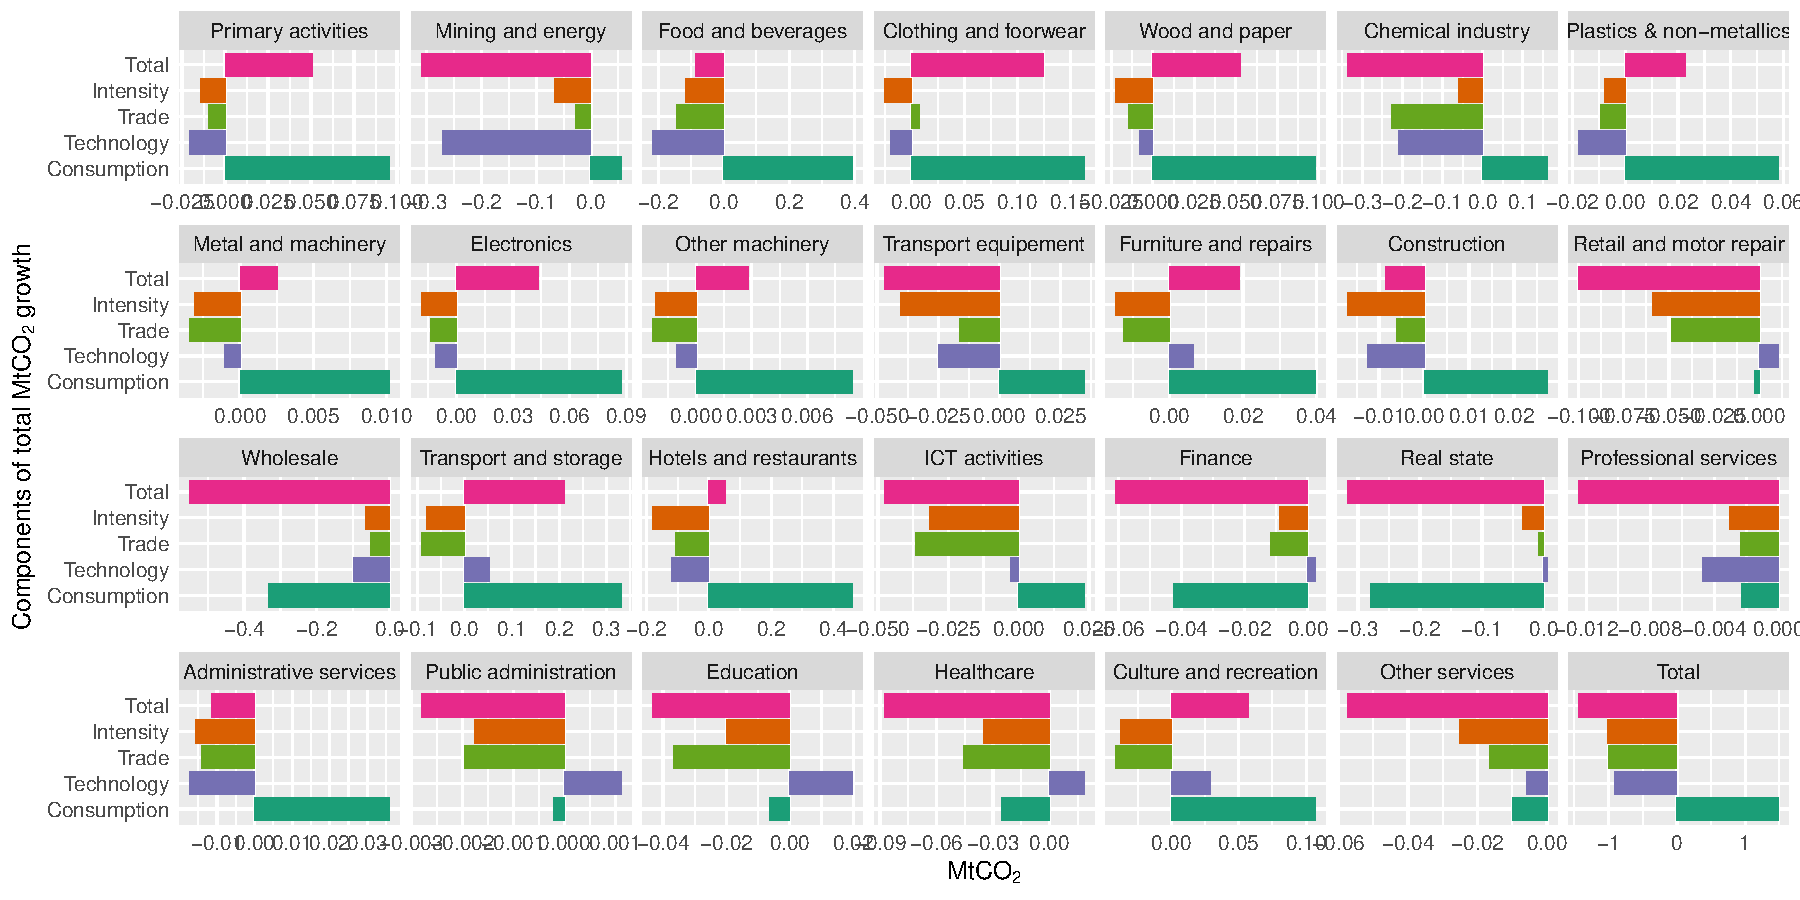
\includegraphics[width=1\textwidth,height=\textheight]{graphics/sda_decomposition.pdf}

}

\caption{\label{fig-sda-decomposition}Structural decomposition of total
Mt\(CO_2\) growth in Madrid into emissions intensity, trade, technology,
and consumption demand contributions for the city of Madrid.
\emph{Source}: Author's own calculations using FIGARO, ES-HBS, and
municipal accounts.}

\end{figure*}%

Figure~\ref{fig-sda-decomposition-cou} shows the full country results
using data from FIGARO. Across countries, we see that regardless of
emissions growing or shrinking, the contribution by the \(\text{CO}_2e\)
intensity of the aggregate economic activity is negative and
considerable with very few exceptions, such as Norway, Cyprus,
Argentina, Brazil, Russia, and Turkey. Trade, on the other hand, tends
to add to total emissions for the majority of countries, most notably
export-oriented economies, such as India, Ireland, Canada, and Norway,
ordered by the proportion of their contribution. Technology tends to
substract from emissions growth, but there are some examples of the
opposite, such as Russia, Cyprus, Lithuania, and Norway. Consumption
demand, however, adds considerably to total emissions, and is in most
cases solely responsible for countries failing to reduce their emissions
despite gains in efficiency, trade or technology. Countries with
negative growth of consumption demand are Argentina, Russia, Turkey,
Australia, Greece, and Brazil. Spain excluding Madrid city displays a
very common pattern: negative contributions by intensity and technology,
but positive by consumption and trade, albeit small in the latter case.
There are 13 countries in this situation that have seen their emissions
declined, most importantly Estonia, Germany, United Kingdom, Denmark,
France, Sweden, Slovenia, and the rest of Spain, and 7 countries with
rising emissions, among which we can highlight India, the rest of the
world, South Korea, Canada, and South Africa. A majority of medium to
large EU countries share the same pattern as Spain. In addition to this
pattern, the city of Madrid benefits also from trade, and only
consumption demand is pushing emissions higher, compensating most of the
emission saved by the other three factors. Even if comparing a capital
city with other countries is unreasonable, it still shows that it is not
on the emissions-intensive end of the country and their neighbours.

If we compare this results with individual industries, we observe a
large degree of heterogeneity that makes aggregate results not
representative of the underlying drivers. The three industries that have
increased their emissions the most in absolute terms are transport and
storage, clothing and foorwear, and culture and recreation, with 210.9,
124.3, and 57.3 \(\text{ktCO}_2e\), respectively. Conversely, public
administration, construction, and administrative services realized the
largest fall in emissions, -11.3, -8.5, and -2.8 \(\text{ktCO}_2e\). In
percentage terms, clothing and foorwear, wood and paper, and electronics
showed the largest increases, and construction, administrative services,
and food and beverages the largest declines. By component, we find no
industry where the contribution of emissions intensity was positive.
Nevertheless, variance in the extent of the reduction is considerable.
From -180.6 \(\text{ktCO}_2e\) in hotels and restaurants to -1.8
\(\text{ktCO}_2e\) in public administration. For the most part, the
negative contribution of trade to emissions growth is smaller than
intensity, but still significant. In particular, professional services,
construction, and clothing and foorwear show a larger contribution to
emissions reduction from trade than intensity. On the other hand, the
effect of technology is modest and mixed, with some sectors adding and
other substracting from total emissions. Noteworthy sectors are
education, culture and recreation, and transport and storage, where
technology outweights intensity and trade. Finally, the contribution of
final consumption is robust and inequivocally positive, with the
exception of education, public administration, and retail and motor
repair, where it declines. Overall, these results indicate that
\(\text{CO}_2e\) emissions have continued to grow due to the strong pull
by consumption demand despite the generalized gains in efficiency,
trade, and technology across a majority of industries along the entire
global value chain supplying to the city's economy.

\begin{figure*}

\centering{

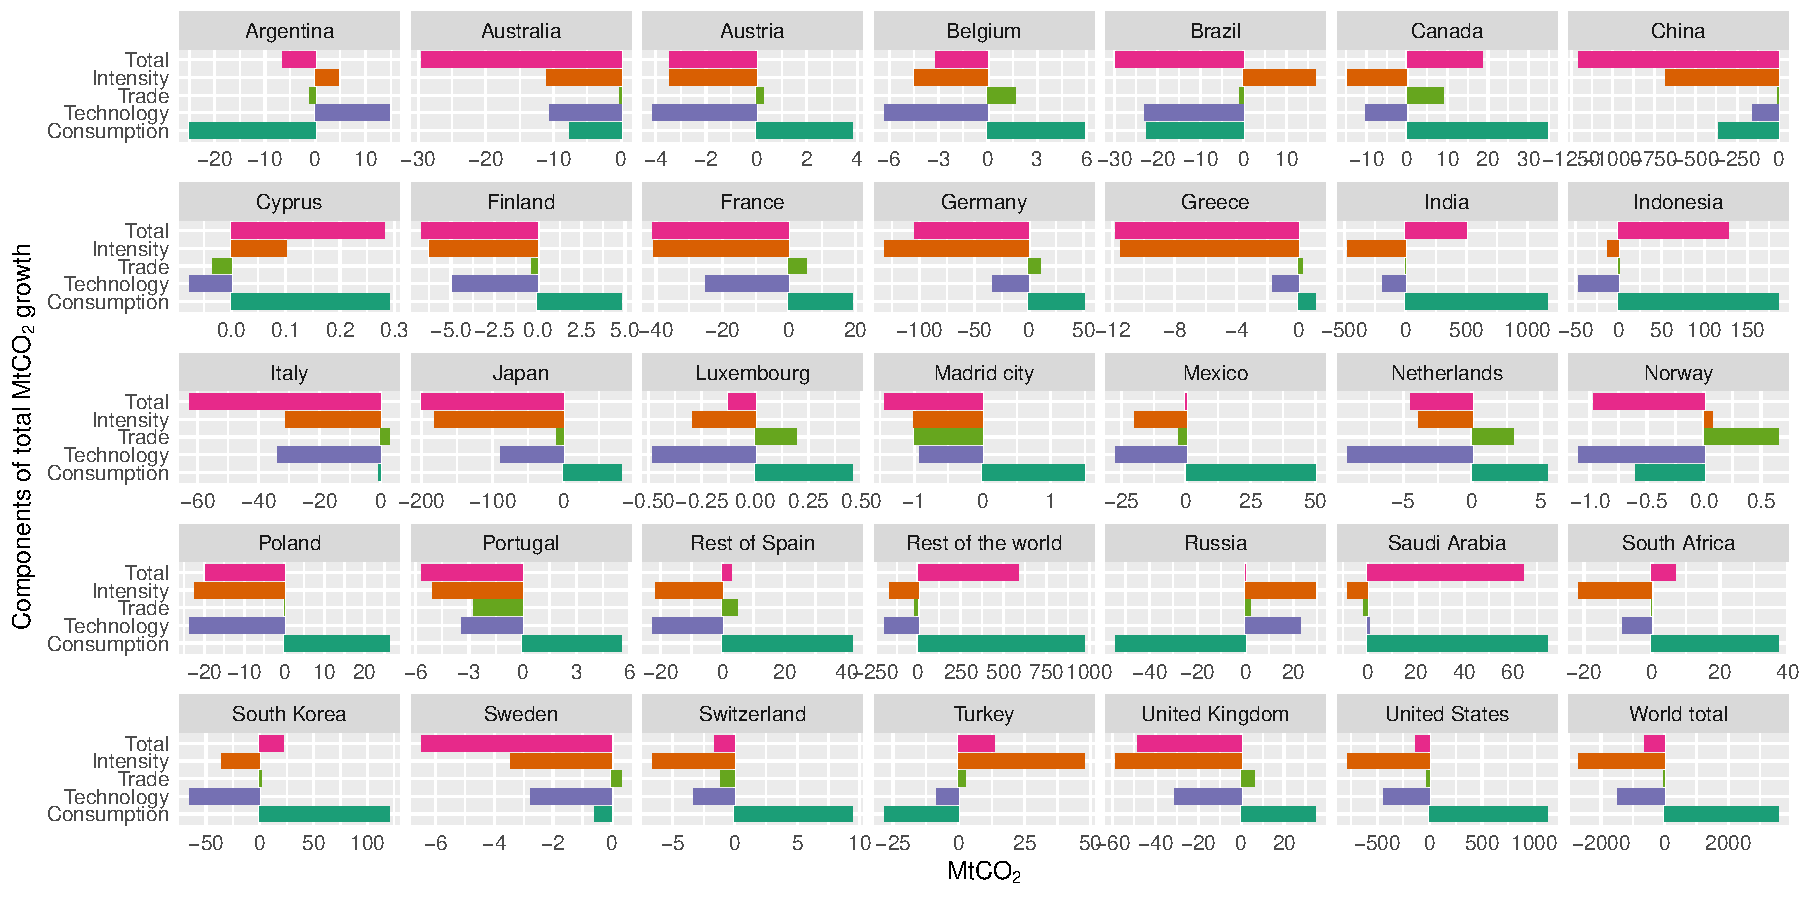
\includegraphics[width=1\textwidth,height=\textheight]{graphics/sda_decomposition_cou.pdf}

}

\caption{\label{fig-sda-decomposition-cou}Structural decomposition of
total Mt\(CO_2\) growth for selected countries into emissions intensity,
trade, technology, and consumption demand contributions for all
countries in the sample. \emph{Source}: Author's own calculations.}

\end{figure*}%%
\begin{figure*}

\centering{

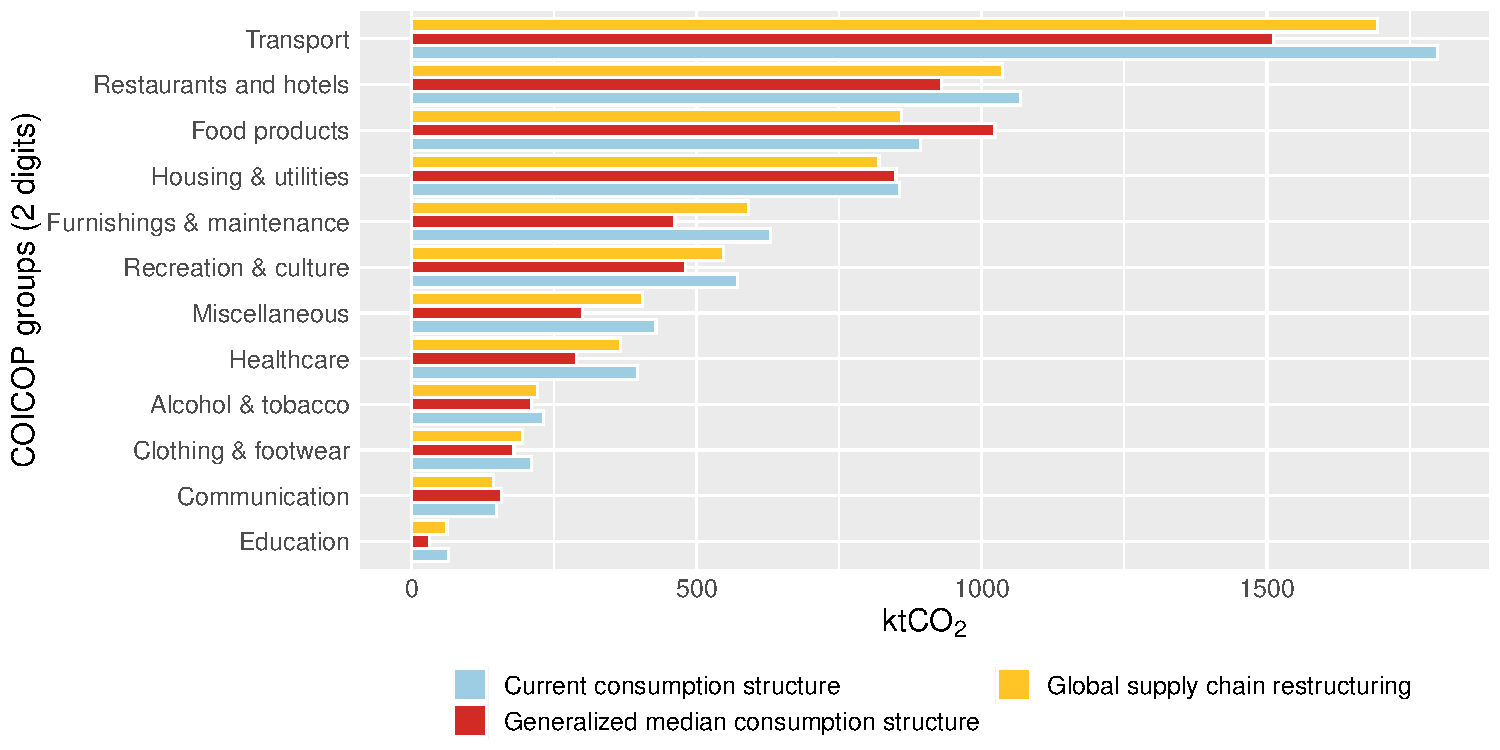
\includegraphics[width=0.9\textwidth,height=\textheight]{graphics/three_scenarios_coicop_CO2_reduction.pdf}

}

\caption{\label{fig-cf-coicopCO2}Total embedded household
consumption-linked emissions from Madrid by consumption purpose before
and after the hypothetical projection of the median consumption
structure, 2019. \emph{Source}: Author's own calculations}

\end{figure*}%

We have observed that consumption strongly constraints or even reverses
the push by efficiency, technology, and trade towards emissions
reduction. By the same token, we can highlight that the contribution by
the trade structure is only modest. An important hypothesis in the
literature, and a environmental talking point, is that supply chain
offshoring had been used as means for pollution evasion by advanced
economies \citep{levinsonUnmaskingPollutionHave2008}, which would
indirectly benefit from shifts in the trade structure towards more
efficient countries. This argument has been challenged in the past
\citep{artoDriversGrowthGlobal2014}, and our results agree with a
relatively modest, and sometimes contradictory, emissions reduction
potential from supply chain restructuring. Consumption demand clearly
shapes the slow pace of decarbonization. Likewise, an important policy
concern is the the potential of re-shoring to enhance mitigation
efforts. To further assess the potential for emissions abatement and as
a way to indirectly highlight the weight of domestic policies, we
simulate three scenarios. From a methodological perspective, this is
implemented, as explained in section \ref{sec-subsec-decomposition}, by
simulating a trade shock to matrix \(\mathbf{C}\), from which we derive
a modified matrix \(\mathbf{A}\) to calculate consumption-driven
emissions following the Equation~\ref{eq-carbon-footprint}. In the first
scenario, we explore the consequences of trade decoupling from
non-Western suppliers by simulating a series of shocks on 10-point
increment intervals to the input supplied by non-Western to Western
countries, which are then substituted by intra-block Western supplies.
For instance, we reduce the supplies of energy products from Saudi
Arabia to France and, at the same time, we proportionally increase the
supply from other Western countries to meet up the trade gap left by
Saudi Arabia. This reallocation of input supplies follows the existing
procurement proportions from other countries in the block, and assumes,
somewhat unrealistically, that firms in Western countries are fully able
to close the import gap in quality, quantity, and price. In addition to
the current 28 EU countries, we include Canada, the United Kingdom,
Japan, and the United States within the Western block. Secondly, we
replicate the same exercise but this time restricting the domestic block
to EU countries, with the purpose of illustrating harsh EU import
restrictions that might be motivated by the desire to avoid carbon
leakage. Finally, we produce an additional simulation in which EU
countries switch from Chinese to US supplies, without affecting any
other intermediate flow in the system. These three simulation scenarios
are inspired by the recent implementation of tariffs and other trade
barriers between the US, the EU, and China, and seeks to explore the
extent to which, if feasible to swap suppliers, emissions will grow or
fall as a result. These scenarios, which affect multiple countries,
illustrate possible reconfigurations of trade that can potentially
impact Madrid's scope-3 emissions.

For the first scenario, we obtain an -7.48\% decline in emissions when
applying a 50\% shock to supplies from non Western countries, from
8655.8 \(\text{ktCO}_2e\) to 8008.5 \(\text{ktCO}_2e\). The main
industries contributing to this decline are food and beverages, mining
and energy, hotels and restaurants, and chemical industry, with a
-4.3\%, -7.6\%, -5.6\%, and -14.4\%. For the second scenario, total
emissions fall down to 7937.4 \(\text{ktCO}_2e\), which is 99.1\% of the
first scenario. We find the same sectors driving the reduction in
emissions, with a -4.4\%, -8.4\%, -6\%, and -18.6\%, respectively.
Lastly, we find that a 50\% shock to trade from China filled in by the
United States has almost no effect with a -0.02\% decline down to 8654.5
\(\text{ktCO}_2e\). There is no difference at the sectoral level to
highlight. In general, the simulation exercises suggest that the ability
of trade policy to have a meaningful impact on total emissions, even
when drastic measures are taken, is very limited. Notwithstanding this,
trade compounds with the evolution of technology and efficiency in the
exporter countries, so it is possible that this may change in the
future.

For the purpose of this simulation using data from 2021, the results
underscore the overwhelming importance of consumption in determining the
slow pace of emissions reduction despite the outstanding gains in
efficiency. In this sense, Figure~\ref{fig-cf-coicopCO2} shows how many
\(\text{ktCO}_2e\) would the city save if we impose the median
consumption structure on the top 50\% of the equivalized spending
distribution. To compare this result with the impact from trade
restructuring, we also include one additional simulation scenario in
which we reduce by 50\% the supplies from all non-EU countries to Madrid
and, conversely, fill the gap with imports from the EU alone.

\section{Discussion and implications}\label{sec-implications}

By projecting urban-level SUTs and deriving an AEA out of the local
inventory we have verified that the speed of the reduction in direct
\(\text{CO}_2e\) emissions in the city of Madrid has remained unmatched
by the evolution of scope-3 emissions during the period 2010-2021. Under
the assumption that the regional proportion of imports plus the national
distribution of international demand constitute a reasonable
approximation to the economic relationship of the city with the outside
world, this paper has quantified the city's consumption-based CF in the
order of 17447 \(\text{ktCO}_2e\) for the city's GDP, from which 2699
\(\text{ktCO}_2e\) are direct emissions. We have also estimated the CF
from the perspective of the residents' total expenditure and direct
activities at 13920.9 \(\text{ktCO}_2e\). In per capita terms, the
average city resident emitted 4193.8 \(\text{kgCO}_2e\) in 2021.

These magnitudes differ from but fall in line with the very few
available estimations. \citet{andradeImplementingCitylevelCarbon2018},
using the PAS2070-DPSC methodology, estimated Madrid's total
\(\text{CO}_2e\) emissions in 2010 at 28160 \(\text{ktCO}_2e\) and 8610
\(\text{kgCO}_2e\) per capita. Whereas direct emissions amount to 7330
\(\text{ktCO}_2e\), Scope-2 and -3 add up to 4740 \(\text{ktCO}_2e\) and
16080 \(\text{ktCO}_2e\), respectively. For 2010, using our approach, we
find wery similar estimations: 27963 \(\text{ktCO}_2e\) for the city's
GDP. On the other hand, C40 Cities quantified the total
consumption-based greenhouse gas emissions for Madrid in 2011 at 47230
\(\text{ktCO}_2e\) and 14770 \(\text{kgCO}_2e\) per capita. However, in
this case we find a substantially lower estimation of 19424.2
\(\text{ktCO}_2e\) driven by household final consumption expenditure.
Nonetheless, at a more disaggregated level distributions are similar.
\citet{andradeImplementingCitylevelCarbon2018} find that all combined
transport industries emit the most at 11440 \(\text{ktCO}_2e\), but they
include also direct emissions by private transport. The industry of food
and drinks is estimated at 3550 \(\text{ktCO}_2e\) and construction
similarly at 3380 \(\text{ktCO}_2e\). Instead of looking at industries,
C40 provides information by consumption purpose. The ranking of sectors
is very similar at 2 digits, but the values are twice as large on
average. The available estimations are few, but, more importantly,
considerably outdated. Comparatively, this paper presents a whole series
groing from 2010 to 2021, in addition to an improved methodology
benefitting from more up to date methodology, an GMRIO framework, and a
formal process of conversion of the local AEI into a fully-fledged AEA.

Hence, we argue that our estimation improves not only the timeliness but
the precision of previous contributions. First, the development of
FIGARO's GMRIO database \citep{remond-tiedrez_eu_2019} and the
methodological progress made in the literature
\citep{cazcarro_linking_2022, wiedmann_concept_2016, corcoles_carbon_2024}
have refined the estimation method and reduced several sources of bias,
such as the more rigorous derivation of the final consumption vector or
international demand from several regions of the world. Crucially, by
parting with the national technology assumption, we have reduced the
weight of some overrepresented carbon-intensive industries, such as
manufacturing, from direct and indirect emissions
\citep{eea_environmental_2013}. Second, the construction of an AEA for
Madrid have fine-tuned our quantification of consumption-based emissions
and improved our understanding of emissions derived from household
activities. Third, our ability to compute more consistent results for
Madrid creates the opportunity for improving the coherence, granularity,
and precision of the estimates such that they may enhance local
mitigation planning. We consider these improvements a definite step
closer to a state of the art CF estimation of the city of Madrid, which
should contribute to the design of credible and effective
decarbonization commitments by the City Council.

In this regard, we derive three main conclusions from Sections
\ref{sec-subsec-results-gdp} and \ref{sec-subsec-results-households}.
First, the geographical distribution of emission sources problematizes
the national assumption used in previous estimations. In 2021, only 15\%
of emissions came from within the city, while the rest of the nation and
the rest of the world contributed 33.1\% and 51.4\%, respectively. The
distribution has shifted slightly since 2010, with the rest of the world
increasing its share from 47.2\% to 51.4\% at the expense of the rest of
the nation, which accounted for 40.1\% of all emissions in 2010.
Furthermore, the ability to break indirect emissions down by industries
and countries reveals both supply chain reconfiguration dynamics, such
as a potentially problematic substitution of imports from China to the
United States, and mitigation bottlenecks in the strong dependence from
certain country's industrial production.

Second, our analysis reveals significant emissions inequality among
Madrid's residents, with age, gender, and income quintile playing
crucial roles. The top 20\% of the spending distribution emitted on
average 11138.2 equivalized \(\text{kgCO}_2e\) in 2021, which is 4.8
times as much as the 2299 \(\text{kgCO}_2e\) emitted by the bottom 20\%.
This distributional gap is due to both level and composition changes in
consumption patterns across income groups. While healthcare and
miscellaneous items show the largest quintile gap, food products and
heating have the lowest. In general, we don't find strong differences by
demographics, with the exception of the education level and partially
the age group of the reference person of the household. Those groupings
that overlap with income differentials tend to display larger variation.
For the most part, emissions inequality is strongly correlated with
income and expenditure inequality. These findings highlight the need for
climate policies that remain sensitive to socio-economic inequalities,
gender differences, and age-shapped consumption patterns.

Third, as shown by our two simulation scenarios for consumption
expenditure and direct household transport emissions, there is a
substantial margin to shrink Madrid's CF by addressing the consumption
and mobility choices of high-income households. Instead of focusing on
the emissions intensity of foreing-supplied goods, our analysis has
highlighted the outstanding potential of domestic policies without
targetting consumption \emph{levels}. For instance, we showed that by
fixing the median consumption structure above the \(50^{th}\) percentile
would produce a total emissions savings of 3688.2 \(\text{ktCO}_2e\) in
2021. This is due to the counter-intuitive result that high-income
groups spend way more on recreational and personal services that poorer
households, which have a considerble indirect emissions footprint. At
the same time, we considered the potential of direct mobility policies
for emissions curbing. If one in every two households in the top five
deciles suppresed their use of private motor vehicles in exchange for
carbon-neutral options for travel, we would save 617 \(\text{ktCO}_2e\)
(-26.7\%). In the extreme and, unfortunately, unrealistic case that this
two policies come to fruition simultaneously, the city's CF will decline
from 13921 \(\text{ktCO}_2e\) to 8538 \(\text{ktCO}_2e\), or by 38.7\%.

Third, our structural decomposition analysis underscores that
consumption is the primary driver of emissions growth, offsetting gains
made through efficiency improvements and technological advancements.
Between 2013 and 2019, Madrid experienced a decline in total emissions
of -1440.3 \(\text{ktCO}_2e\). This result is driven by a 1487.5
\(\text{ktCO}_2e\) increase of final consumption, offset by decreases of
-9.4\%, -9.2\%, and -8.5\%, which are driven by efficiency improvements,
changes in trade structure, and technological advancements,
respectively. While the smallest contribution comes from changes to the
technique of production, the larger emissions savings are realized
thanks to efficiency gains. However, these gains are being largely
offset by increases in consumption, particularly among higher-income
groups. This underscores the need for policies that do not only promote
technological progress and efficiency gains but also address consumption
patterns. Our simulation exercises further support this, showing that
imposing the median consumption structure on the top 50\% of the
equivalized spending distribution would amount to a reduction of 3688.2
\(\text{ktCO}_2e\) (26.7\%) in 2019, with the largest reductions in
transport services, hotels and restaurants, and recreation and culture.

We find that these conclusions bear two main policy implications for
city decarbonization plans. On the one hand, the global nature of
Madrid's CF, whose trans-bordering emissions reached 85\% in 2021,
highlights the need to consider the constraints imposed by global supply
chains on emissions curbing plans. Policymakers should promote
sustainable procurement practices by encouraging decarbonization efforts
of key suppliers, even if the ability to enforce regulation on foreign
firms might prove limited and the emissions savings low to moderate.
Conversely, the observed shift in emissions from China to the United
States between 2010 and 2021, coupled with the outstanding fall in
Chinese emission factors, calls into question any long-term plans that
do not monitor decarbonization strategies across the world. Particularly
if it tries to make virtue out of necessity from emerging geopolitical
rivalries between blocks. For the most part, any serious attempt at
targeted mitigation policy needs to weigh in on the complicated balance
between carbon intensity and growth-pulling industries in highly
tertiarized economies. Hotels and restaurants is a case in point.

On the other, we emphasize the need to prioritize consumption in
Madrid's mitigation efforts, with a particular focus on high-income
households. Our analysis reveals that these groups generate
significantly more emissions, especially due to their intense use of
private transportation and recreational spending. Targeted policies
aimed at reducing emissions from private vehicle use among these
high-emitting groups could yield substantial reductions. This could
involve a combination of incentives for electric vehicle adoption,
improvements in public transport infrastructure, and measures to
discourage private car use in urban centers. Additionally, policies
addressing consumption patterns of high-income households could lead to
significant emissions reductions. Our simulation shows that imposing the
median consumption structure on the top 50\% of households could reduce
emissions by 11.9\%, which illustrates the potential impact of such
targeted interventions. Furthermore, the city's ability to enforce and
implement these policies is crucial. Given the significant emissions
inequalities observed, policies should be designed with social equity in
mind. Measures that disproportionately burden low-income groups or fail
to address the outsized contributions of high-income groups are likely
to be both less effective and less socially acceptable. This calls for a
nuanced approach that could involved a combination of awareness
campaigns, education programs, and fiscal policies to discourage
carbon-intensive consumption choices, particularly among high-income
groups. While our analysis shows that efficiency improvements and
technological advancements are contributing to emissions reductions,
these gains are being largely offset by increases in consumption. Our
main recommendation for Madrid's mitigation policies is to go beyond
traditional supply-side measures and actively address household
consumption patterns, which seem to stirr in the opposite direction of
decarbonization.

\section{Conclusions}\label{sec-conclusions}

This paper has presented the most rigorous quantification of the 3-scope
CF of the city of Madrid to date, which is a crucial input to mitigation
planning that has been missing. Additionally, it lays down relevant
implications for specific policy designs. We provide sectoral data and
household distributional information that opens the space for targeted
and more sensitive interventions. The empirical results developed in the
paper showed the importance of global supply chain constraints and
possible trade shocks in monitoring progress of climate change
mitigation. Nonetheless, the evidence collected leads to the
recommendation to focus on consumption demand and, from the perspective
of households' direct emissions, on private mobility. The latter can be
seen to yield a disproportionate amount of emissions reduction, but
consumption demand interventions emerge also as a potentially fruitful
policy avenue. In this sense, a primary target for maximum emission
savings should be high-emitting groups, which are strongly correlated
with high-income households. Most importantly, our methodology and data
compilation process lend themselves easily to periodic updates of the
main estimates as new information becomes available, potentially
becoming part of a timely monitoring dashboard for interested
stakeholders.

These results show four main limitations, which create several research
opportunities. Firstly, the regional series is limited to a six-year
period from 2013 to 2019, which we extend using non-survey techniques to
a longer series (2010-2021), mostly limited by the availability of the
local emissions inventory. While RSUTs are published with a four-year
gap, FIGARO is released with a narrower two-year one. Although
coefficient projections add uncertainty, extending the time seires
aligns with the recent emphasis on timeliness in statistical production
\citep[p.~190]{oecdOECDHandbookCompilation2024}. Secondly, urban
economies have a few distinct structural characteristics whose further
study could improve the projections made to derive the AEA and IOTs.
Specifically, properly representing a highly tertiarized economy, with
minimal agricultural production, may benefit from the inclusion of
additional information and estimation techniques
\citep{zheng_entropy-based_2022}. Thirdly, more research is needed to
understand the possibilities to exploit the distributional carbon gaps
identified in Section~\ref{sec-subsec-results-households} for mitigation
policy. Consumption was identified as a more relevant driver of total
emissions than the trade structure, but carbon inequality and
transportation are not only the two most important mitigation vectors,
but probably the two least difficult to enforce. Lastly, uncertainty
evaluation has remained mostly unaddressed in the literature and the
official estimations made by the designated statistical agencies
\citep{eea_environmental_2013}. Although challenging, additional
sensitivity analysis and uncertainty calculations could increase the
reliability of the results presented in this paper, which we seek to
continue developing.

\textbf{Authorship contribution statement}: \textbf{Jacobo Ferrer}:
conceptualization, research, programming, writing, review \& editing,
visualization, formal analysis, validation, methodology, data curation.
\textbf{Sergio Alvarez}: funding acquisition, review \& editing, climate
science validation.

\newpage

\section*{References}\label{references}
\addcontentsline{toc}{section}{References}

\renewcommand{\bibsection}{}
\bibliography{Paper_references.bib}

\newpage

\section*{Appendix}\label{appendix}
\addcontentsline{toc}{section}{Appendix}

\begin{table}[!ht]
\centering\begingroup\fontsize{10}{12}\selectfont
\vspace{-0.25cm}
\begin{tabular}[t]{cl}
\toprule
NACE (rev.2) & Industry definition\\
\midrule
A & Primary activities\\
B\_E & Mining and energy\\
C10\_C12 & Manufacturing of food and beverages\\
C13\_C15 & Manufacturing of clothing and foorwear\\
C16\_C18 & Manufacturing of wood and paper\\
C19\_C21 & Manufacturing of chemical industry\\
C22\_C23 & Manufacturing of plastics \& non-metallics\\
C24\_C25 & Manufacturing of metal and machinery\\
C26\_C27 & Manufacturing of electronics\\
C28 & Manufacturing of other machinery\\
C29\_C30 & Manufacturing of transport equipement\\
C31\_C33 & Manufacturing of furniture and repairs\\
F & Construction\\
G46 & Wholesale\\
G45YG47 & Retail and motor repair\\
H49\_H53 & Transport and storage\\
I & Hotels and restaurants\\
J58\_J63 & ICT activities\\
K64\_K66 & Finance\\
L & Real state\\
M69\_M75 & Professional services\\
N77\_N82 & Administrative services\\
O84 & Public administration\\
P85 & Education\\
Q86\_Q88 & Healthcare\\
R90\_R93 & Culture and recreation\\
S94\_S96 & Other services\\
T & Domestic services\\
\bottomrule
\end{tabular}
\endgroup{}
\vspace{-0.25cm}
\caption{Industry classification adapted to city aggregation (NACE rev.2).}
\end{table}

\begin{table}[!ht]
\centering\begingroup\fontsize{10}{12}\selectfont
\vspace{-0.25cm}
\begin{tabular}[t]{lllcc}
\toprule
Code & Heading & Unit & Factor\\
\midrule
04521 & Gas (main dwelling) & $m^3$ & 1.919\\
04522 & Gas (other dwellings) & $m^3$ & 1.919\\
04523 & Liquefied gas (main dwelling) & kg & 2.966\\
04524 & Liquefied gas (other dwellings) & kg & 2.966\\
04531 & Liquid fuel (main dwelling) & l & 2.855\\
04532 & Liquid fuel (other dwellings) & l & 2.855\\
04541 & Coal (main dwelling) & kg & 2.239\\
04542 & Coal (other dwellings) & kg & 2.239\\
04548 & Other solid fuels (main dwelling) & kg & 3.109\\
04549 & Other solid fuels (other dwellings) & kg & 3.109\\
07221 & Diesel & l & 2.520\\
07222 & Gasoline & l & 2.249\\
07223 & Other fuels & l & 2.213\\
\bottomrule
\end{tabular}
\endgroup{}
\vspace{-0.25cm}
\caption{Direct emissions factors in $kgCO_2$ per unit of energy good generated by household activities (5-digit ECOICOP). \textit{Source}: Direct emissions factors and conversion of $m^3$ into kWh obtained from MITECO (2023).}
\end{table}






\end{document}
